\chapter{Predizione della struttura di proteine}

Il protein folding problem ha sia guidato che tratto beneficio dagli avanzamenti nei metodi sperimentali e computazionali\supercite{dill2008protein}. Uno dei maggiori obiettivi della biologia computazionale è proprio il Protein Structure Prediction (PSP), ovvero la predizione della struttura nativa tridimensionale di una proteina a partire dalla sua sequenza amminoacidica. Il PSP è il problema opposto al \textit{protein design} (la progettazione di nuove sequenze proteiche aventi delle specifiche attività).

\par Grazie al CASP\footnote{Critical Assessment of Structure Predictions, vedi la sezione \ref{sec:CASP}.}, alla crescita dei database sulle proteine, allo sviluppo dei metodi per omologia, di allineamento di sequenze e all'utilizzo del Deep Learning, i metodi computazionali hanno registrato incredibili progressi, come il livello raggiunto da AlphaFold può dimostrare. 

\par La predizione della struttura di proteine è uno strumento fondamentale: in medicina per la comprensione delle malattie da misfolding, nell'industria farmaceutica per risparmiare anni di laboriosi e costosi esperimenti correntemente richiesti per lo sviluppo di un singolo farmaco (\textit{drug design}), in biotecnologia per il design di nuovi enzimi e in generale per acquisire maggior conoscenza sul protein folding in tutti i suoi lati.

\section{Metodi e strumenti informatici}

La piccola percentuale di strutture determinate e il gap che continua a crescere con le sequenze conosciute (vedi sotto la sezione \ref{sec:database}) è una conseguenza della lentezza e della dispendiosità dei metodi sperimentali (e in parte anche dei progressi delle tecnologie di sequenziamento). I metodi computazionali, significativamente più veloci ed economici, potrebbero fornire una possibile soluzione a questo problema.

\subsection{Workflow e classificazione dei metodi per il PSP} \label{sec:workflow-psp}
{

Lo sviluppo di metodi computazionali per la predizione della struttura di proteine si è sviluppato lungo due percorsi complementari, che si concentrano sulle \textit{interazioni fisiche} o sulla \textit{storia evolutiva}. Esistono quindi due \textit{paradigmi fondamentali} per affrontare il problema:
\begin{itemize}
	\item paradigma \textit{ab initio}
	\item paradigma \textit{data-based}
\end{itemize}

Il paradigma \textit{ab initio} (o \textit{de novo}) si basa su un approccio puramente fisico, nel quale la struttura è predetta da zero simulando principi fisici. In questo paradigma si integra fortemente la comprensione attuale delle forze molecolari trainanti, in simulazioni termodinamiche e/o cinetiche della fisica delle proteine, o in approssimazioni statistiche della stessa.

\par Nel paradigma \textit{data-based} invece si fa uso di informazioni estratte da database di sequenze o strutture di proteine. 

\par Le proteine che esistono in natura oggi si sono sviluppate attraverso lunghi processi evolutivi, progredendo attraverso mutazioni casuali e selezione naturale. La rivoluzione genetica degli anni '50, consentendo la determinazione delle sequenze amminoacidiche, ha permesso il nascere di metodi di confronto delle sequenze. È per questo che si possono ricavare informazioni sulla struttura 3D di una sequenza amminoacidica cercando altre proteine con proprietà nella sequenza simili e una struttura nota.\\

\par È bene chiarire sin dall'inizio che metodi basati totalmente sul primo paradigma non sono computazionalmente trattabili. Per questa ragione, i metodi odierni per la PSP di sequenze senza struttura nota, sono sempre in qualche misura \textit{data-based}. Possono essere quasi totalmente basati sui dati come nel caso della modellazione per \textit{omologia} e \textit{fold recognition} oppure parzialmente basati sui dati negli altri casi.

\par L'utilizzo, anche parziale, di tecniche \textit{data-based} è necessario per guidare la ricerca nello spazio conformazionale tramite rappresentazioni più grossolane, in modo da superare il paradosso di Levinthal.

\par Varie osservazioni evolutive e strutturali supportano questo approccio. Si è visto che la struttura è più conservata della sequenza: un'identità anche solo del 50\% può implicare un'identità di ripiegamento ed è possibile ricavare informazioni da mutazioni coevolute.

\par L'approccio \textit{data-based} è anche supportato dall'osservazione che, sebbene il numero di famiglie di proteine multi-dominio cresca rapidamente, la scoperta di nuovi domini singoli sembra stabilizzarsi. Ciò suggerisce che la maggioranza delle proteine possa ripiegarsi in un numero limitato di domini strutturali, forse non più di 10 000 o 20 000. Per molte famiglie a singolo dominio la struttura di almeno un membro è conosciuta: si stima che ciò permetta di avere informazioni su più di 3/4 delle sequenze nei database\supercite{alberts2018essential}. \\

\par Una \textit{pipeline} standard per la previsione della struttura delle proteine è basata su fasi di previsione intermedie, nelle quali vengono dedotte delle astrazioni che, risultando più semplici della struttura 3D completa, rivelano delle informazioni importanti per guidare le successive ricerche e modellazioni. Queste informazioni possono essere chiamate "annotazioni della struttura delle proteine" (Protein structure annotations, PSA). Le annotazioni sono divise in 2 categorie a seconda delle informazioni che forniscono:
\begin{itemize}
	\item \textit{Annotazioni 1D}: informazioni sulla backbone, caratteristiche strutturali locali (es. formazione di strutture secondarie, accessibilità al solvente)
	\item \textit{Annotazioni 2D}: vincoli spaziali (es. contact map)
\end{itemize}

\begin{figure}[!htb]
	\centering
	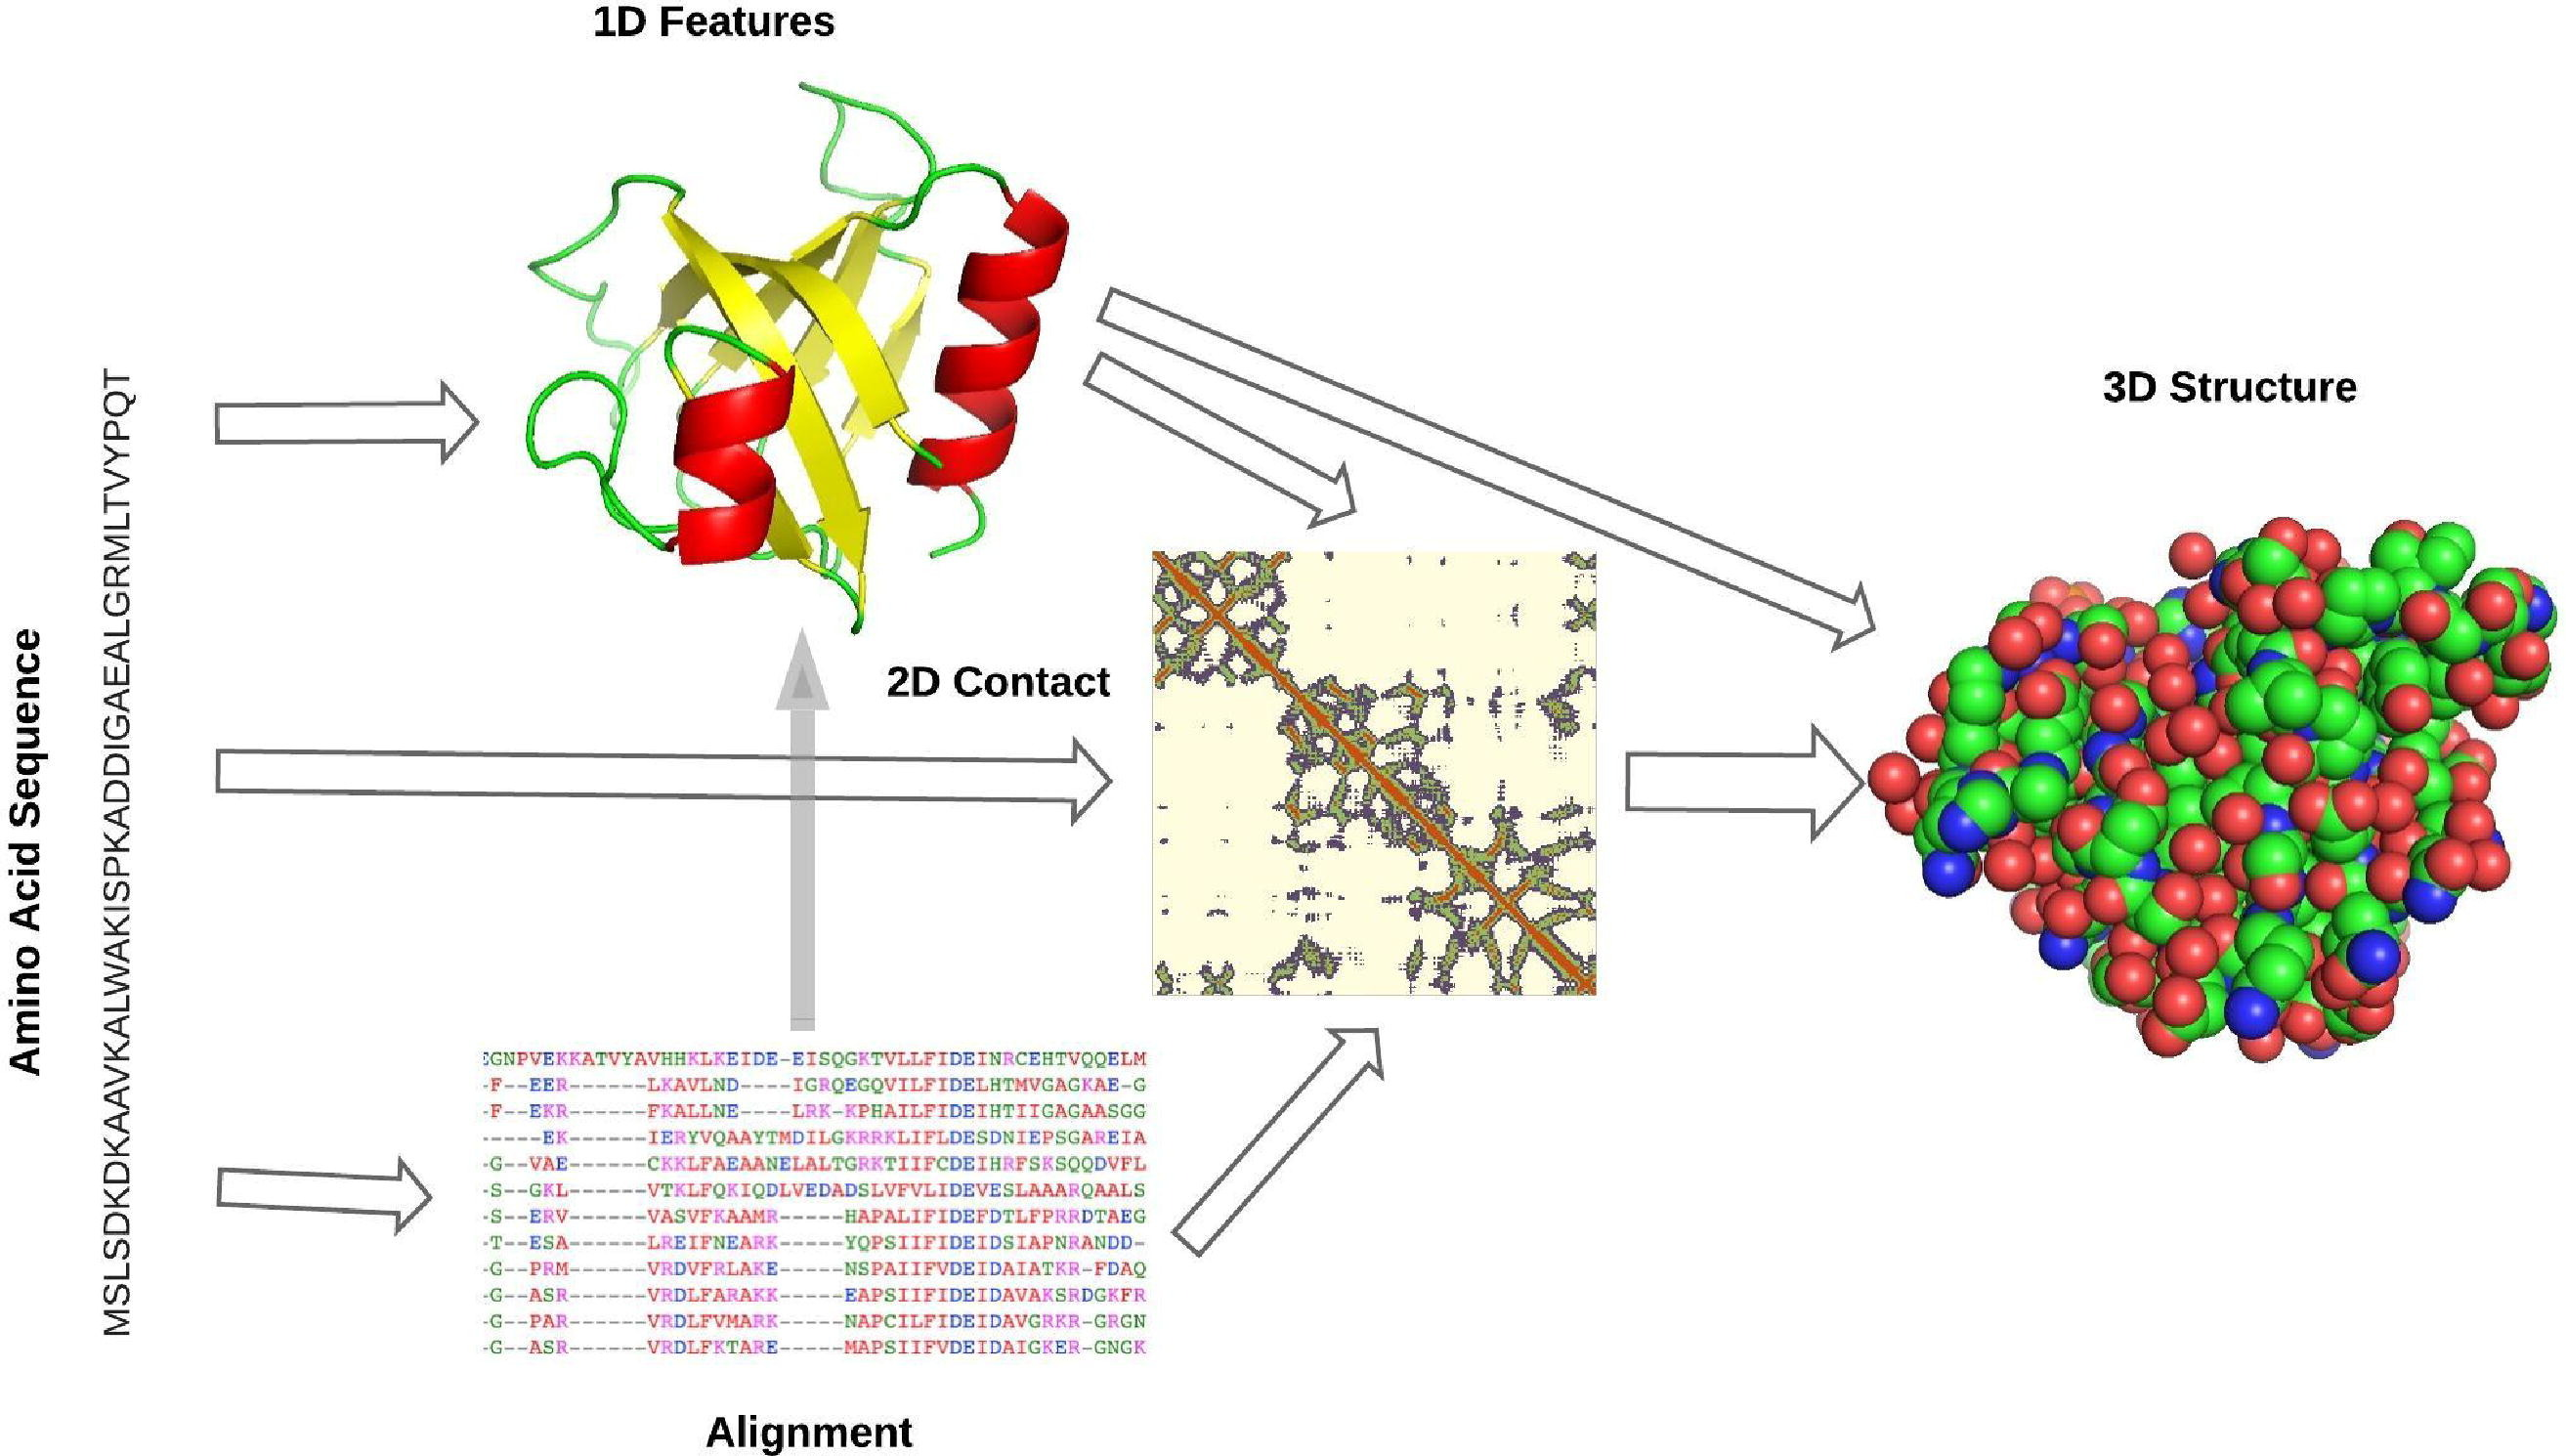
\includegraphics[scale=1]{images/psa.jpg}
	\caption{Pipeline generica per la predizione della struttura 3D di una proteina. Questo schema vuole mettere in risalto gli step intermedi relativi alle annotazioni. Fonte\cite{torrisi2020deep}}
	\label{fig:psa}
\end{figure}

Ci sono due possibili situazioni in cui ci si può trovare quando si vuole modellare una proteina: si riesce a trovare almeno una proteina omologa (o con caratteristiche simili) oppure no. Nel primo caso la struttura trovata verrà chiamata \textit{template} e si affronterà una predizione di tipo \textit{template-based modeling} (TBM), più semplice, mentre nell'altro caso si affronterà una predizione \textit{template-free modeling} (FM).\\


\par Come già accennato, nel panorama attuale molti degli approcci oggi utilizzati per il PSP sono prevalentemente \textit{data-based}: i metodi puri \textit{ab initio} vengono raramente utilizzati per la predizione della struttura di proteine (per ragioni che verranno spiegate in dettaglio nella sezione \ref{sec:ab-initio}). Tuttavia, nella pratica, alcune intuizioni del paradigma \textit{ab initio} vengono usate in metodi prevalentemente \textit{data-based}, ad esempio la funzione euristica di valutazione che simula il campo di forza per calcolare l'energia potenziale. Le varie tecniche vengono utilizzate in combinazione: non vi è una singola tecnica principale e i metodi migliori sono proprio quelli che riescono ad integrare vari approcci. \\

\par  Quando si ha di fronte una sequenza di una proteina senza struttura nota e si vuole predire la sua forma tridimensionale, un metodo per il PSP attuale agirebbe nel seguente modo (vedi fig. \ref{fig:fm-tbm})\footnote{Ogni argomento o metodo citato verrà spiegato nel dettaglio successivamente, in questa sezione l'obiettivo è di fornire una visione globale degli argomenti.}:

\begin{figure}[!htb]
	\centering
	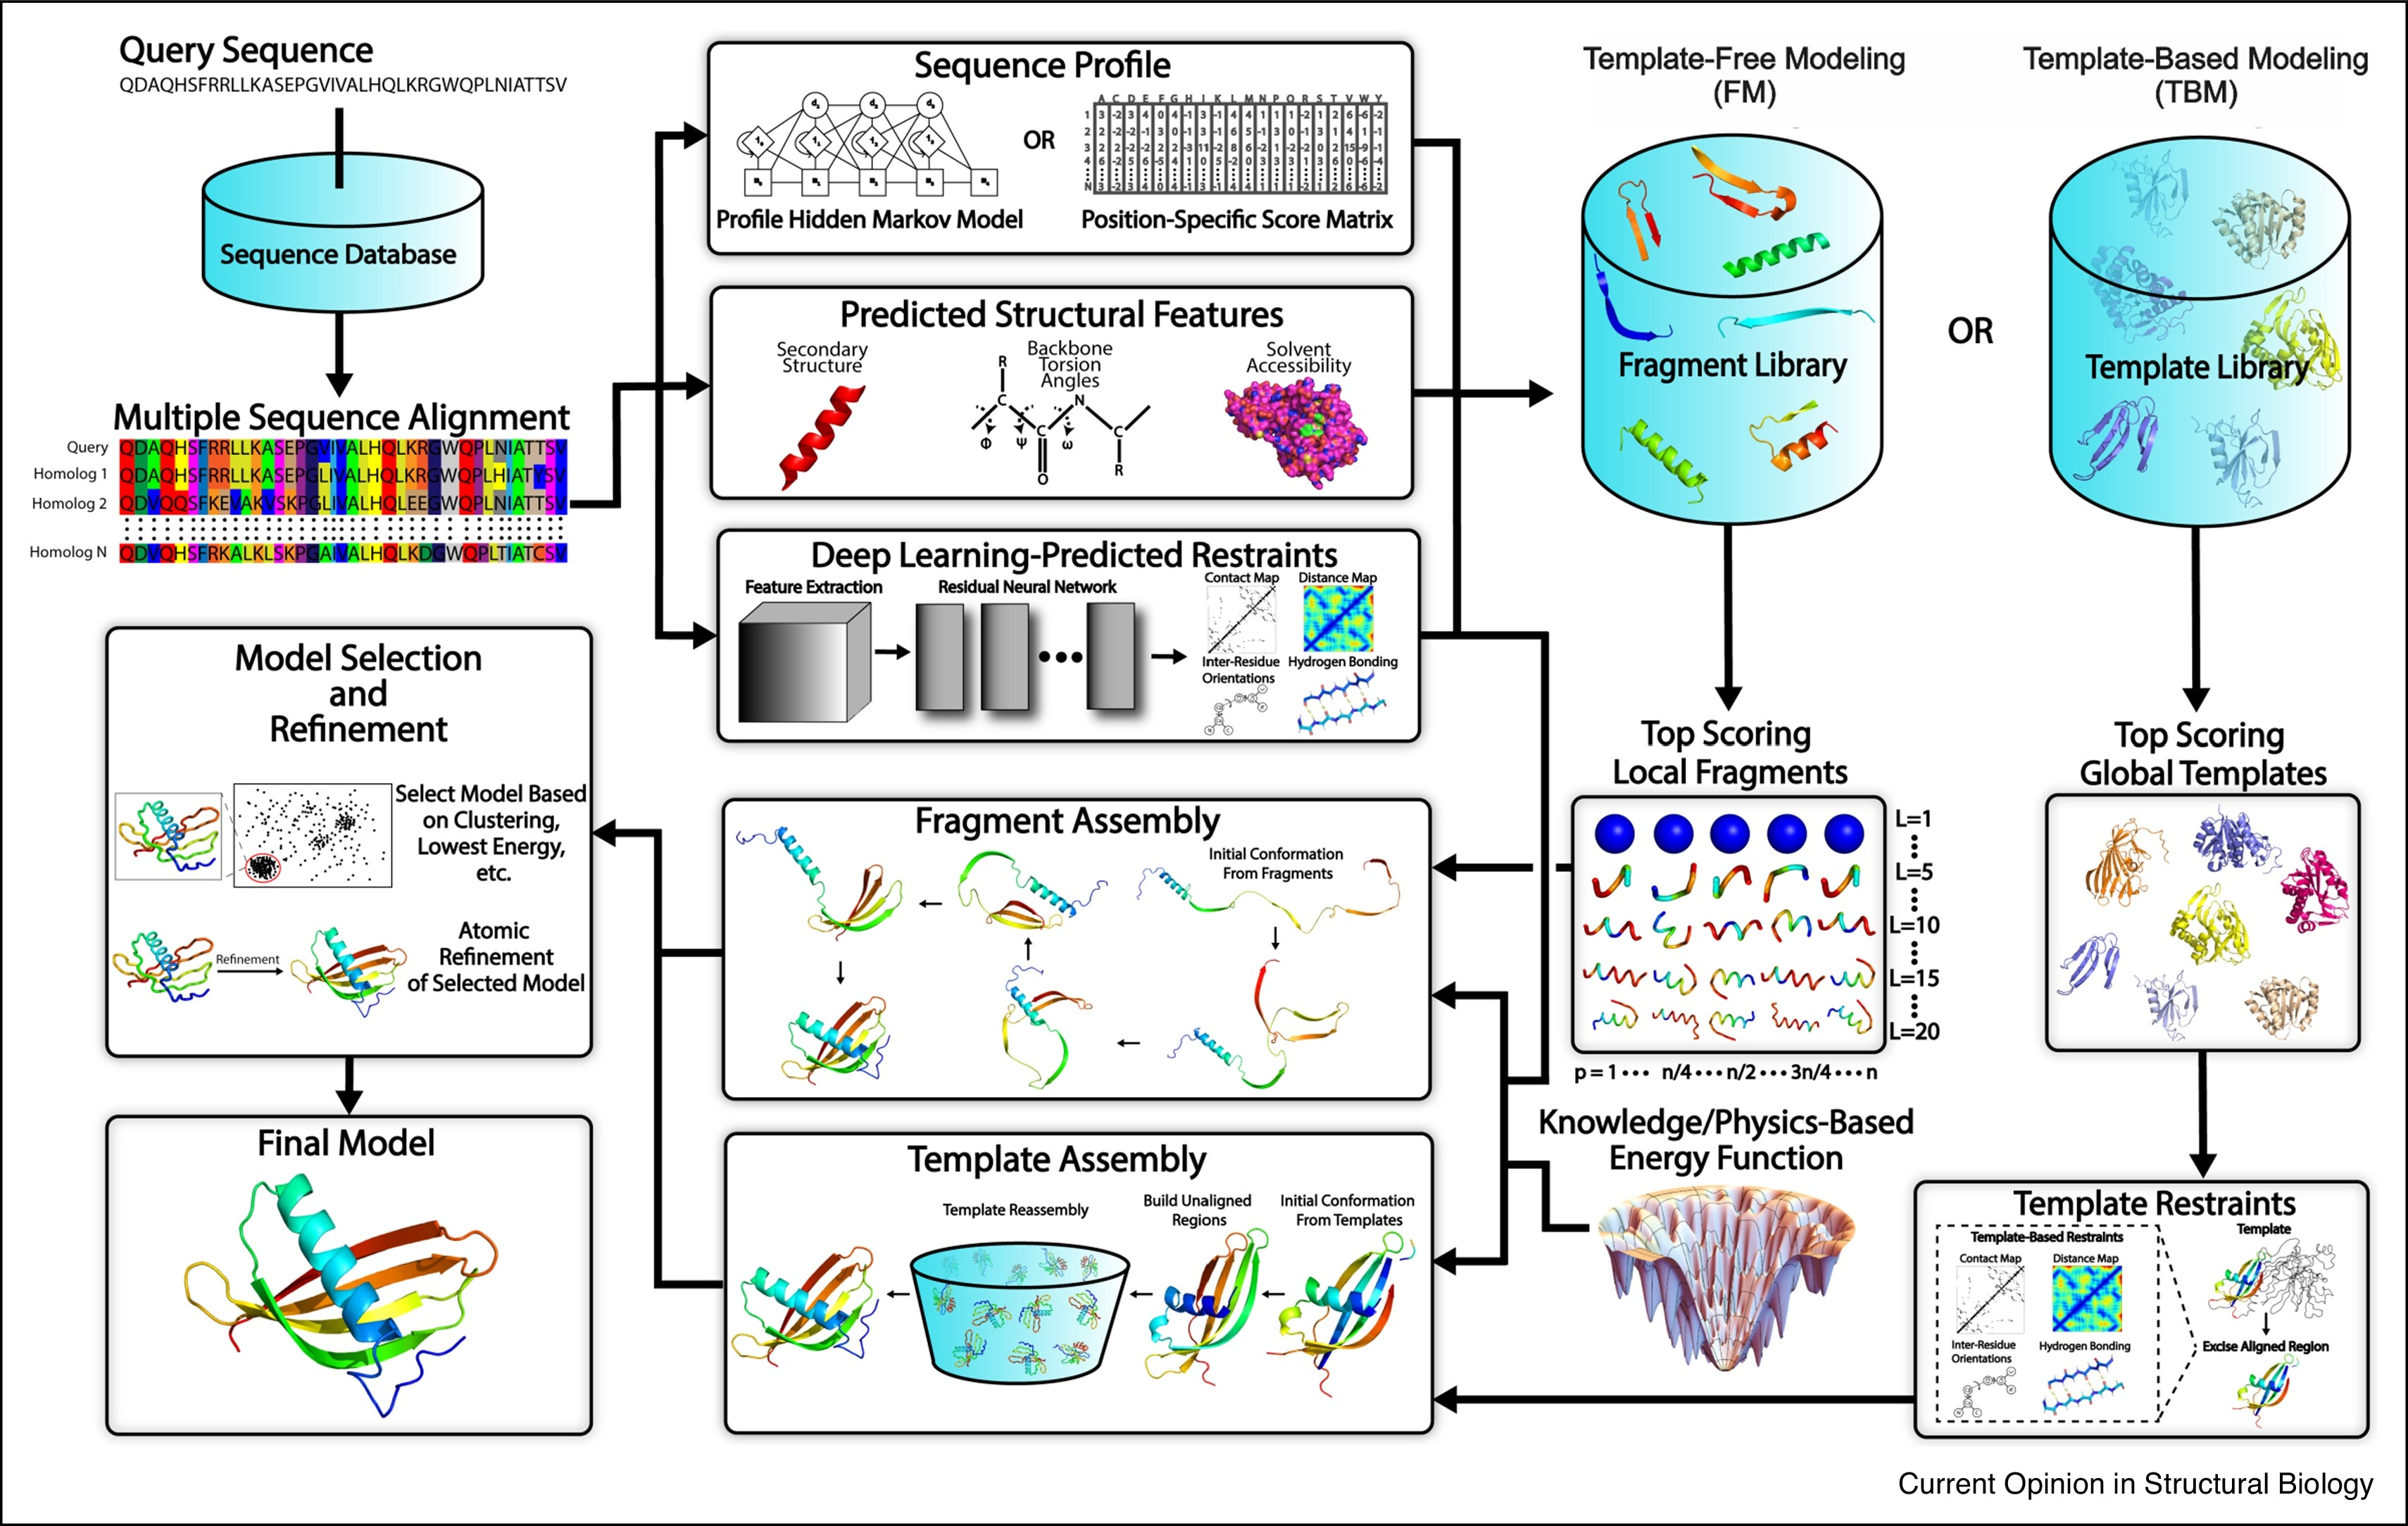
\includegraphics[scale=0.95]{images/FM-TBM.jpg}
	\caption{Step tipici negli approcci al PSP di tipo TBM e FM. Fonte\cite{pearce2021deep}}
	\label{fig:fm-tbm}
\end{figure}

\begin{enumerate}
	\item viene generata una MSA per ottenere informazioni evolutive ed	identificare sequenze omologhe
	\item viene profilata la sequenza, sfruttando anche i risultati dell'MSA, e viene usata per dedurre le annotazioni 1D e 2D
	\item viene scelto il tipo di modellazione adeguato
	\item vengono assemblati i frammenti o i template
	\item viene scelto il modello fra vari candidati, che sarà poi raffinato a livello atomico
\end{enumerate}

\par Nel 1° passo l'obiettivo è ottenere informazioni evolutive che serviranno sia per identificare sequenze omologhe che per dedurre le annotazioni. Se si riesce a trovare almeno una proteina omologa allora sarà possibile procedere alla \textit{modellazione per omologia} (\textit{homology modeling}). \\

\par Nel 2° passo si applicano delle deduzioni sulla sequenza target al fine di ricavare delle annotazioni sulla struttura, per due scopi:
\begin{itemize}
	\item impostare dei vincoli spaziali e strutturali per guidare la modellazione
	\item nel caso in cui non siano state trovate proteine omologhe: per identificare template globali al fine di applicare protocolli di \textit{fold recognition}; se non se ne trovano, tali informazioni verranno utilizzate per valutare i frammenti nella ricerca all'interno di una \textit{fragment library}
\end{itemize}

\par Si rientrerà nel caso del TBM sia che venga eseguita una modellazione per \textit{omologia} che una modellazione basata sul \textit{fold recognition}.
Si rientra invece nel caso del MF quando non si riescono a trovare dei template globali. In questo caso vengono principalmente utilizzate tecniche di modellazione \textit{fragment-based}, ovvero basate su frammenti di proteine che verranno poi integrati. Nel 3° passo, a seconda che ci si trovi nel caso TBM o MF vengono attuate le rispettive modellazioni.\\ 

\par Nel 4° passo l'assemblaggio è eseguito sotto la guida di una funzione euristica del campo di forza, che può essere \textit{energy-based} e/o \textit{knowledge-based}, combinata con una rete neurale profonda per la predizione di determinate caratteristiche. Nel caso di una modellazione TBM si hanno anche delle restrizioni spaziali sul modello. Vengono utilizzate tecniche specifiche per regioni non allineate, come i loop (\textit{loop modeling}). \\

\par Nel 5° passo vengono valutati i modelli, viene eseguita una valutazione della qualità (\textit{quality assessment, QA}) stimando l'accuratezza del modello (\textit{estimation of model accuracy}, \textit{EMA}) e infine viene eseguito il raffinamento. Tipicamente viene scelto il modello con minore energia.

\subsubsection{Nota sulla classificazione dei metodi}

La predizione della struttura di proteine è stata ed è tutt'ora un campo in evoluzione. Per tale ragione risulta difficile classificare e raggruppare i metodi in nette categorie. Agli albori i metodi erano divisi in \textit{ab initio} e \textit{comparative modeling}. Oggi il confine non è più così marcato (come si è potuto vedere dalla panoramica nella sezione precedente). Il CASP divide la modellazione in due classi principali in base alla difficoltà: TBM ed FM\supercite{kryshtafovych2021critical}, in base all'utilizzo o meno di informazioni ricavate da template (proteine con struttura 3D nota). 

\par Nonostante questa divisione possa risultare efficace, in questo lavoro si è ritenuto opportuno seguire una classificazione diversa, che provasse a delineare invece le idee alla base degli approcci odierni e raggrupparli in più livelli secondo questo principio. La motivazione risiede nel fatto che nessun metodo preso singolarmente può dare risultati soddisfacenti: negli anni si è assistito infatti ad un utilizzo combinato dei tanti metodi trovati sfocando sempre più i margini fra le categorie. Tutto questo ha creato confusione ed un utilizzo improprio dei termini. Come si vedrà, \textit{ab initio} indica il "puro" approccio fisico, mentre con la divisione operata dal CASP si tende ad utilizzare come sinonimi \textit{ab initio} e \textit{template-free modeling}\footnote{Un esempio è in \fullcite{torrisi2020deep}. Nonostante ciò è proprio da tale lavoro che si è preso spunto per l'idea delle annotazioni.}, cosa che, in fase di stesura della tesi, è stata reputata equivoca e forse addirittura erronea. Allo stesso tempo i metodi si sono evoluti negli ultimi anni, specialmente con l'avvento del Deep Learning, e le vecchie classificazioni \footnote{Compresa quella di \fullcite{kessel_ben-tal_2018}, su cui il presente capitolo si basa in parte, precisamente sul capitolo 3.4.} non rispecchiano più l'attuale struttura dei metodi usati. Si è deciso di focalizzare l'attenzione sulla struttura dei metodi per il PSP odierni e da qui provare ad astrarre verso l'alto. Si è scelto per tale ragione di dividere la fase di annotazione da quella di modellazione e di rimarcare la differenza basilare tra i due grandi paradigmi per il PSP. Il quadro di riferimento è il \textit{workflow} della figura \ref{fig:fm-tbm}, che delinea la struttura tipica di un metodo attuale (tralasciando i metodi end-to-end come AlphaFold2). 

}

\subsection{Soft computing e deep learning}

Nel corso degli anni il PSP è stato affrontato anche con approcci di \textit{soft computing}. Si sta parlando di approcci perlopiù \textit{data-based}. I principali metodi di \textit{soft computing }utilizzati fanno capo a queste tecniche\supercite{marquez2015soft}:

\begin{itemize}
	\item Machine Learning:
	\begin{itemize}
		\item ANN (Artificial neural network)
		\item SVM (Support vector machines), es. SVM-SEQ 
		\item k-Nearest Neighbors
		\item linear regression
		\item HMM (Hidden Markov Models)
		\item Support vector regression
	\end{itemize}
	
	\item EC (Evolutionary computing), es. MECoMaP
	\item approcci \textit{statistici}, basati principalmente sull'omologia e sul fold recognition
	\item modelli \textit{matematici}, come un adattamento della programmazione lineare intera
\end{itemize}

I limiti della computazione evolutiva sono: la difficoltà di trovare un criterio di arresto e la possibilità di convergere verso un massimo locale come risultato di una configurazione sfavorevole dei parametri. Utilizzando questa tecnica è necessario tenere conto di una corretta scelta della rappresentazione del problema, della funzione fitness, della dimensione della popolazione e del tasso degli operatori genetici. Ad esempio, una piccola dimensione della popolazione può far sì che l'EA non possa esplorare lo spazio sufficiente per trovare una soluzione corretta.

\par Come limiti della tecnica SVM invece si può parlare del fatto che i modelli del kernel overfittino il criterio di selezione del modello, della difficoltà nella selezione dei parametri ottimali della funzione del kernel e della complessità algoritmica e gli ampi requisiti di memoria nei compiti su larga scala.

\par Le reti neurali invece offrono un elevato grado di flessibilità, nonostante la codifica dei dati di input necessariamente restringa l'insieme delle possibili informazioni. Oltre ai vettori di input codificanti coppie di amminoacidi è possibile includere neuroni con informazioni aggiuntive, come la lunghezza della sequenza, valori di idrofobicità dell'ambiente o informazioni evolutive. Le reti neurali presentano comunque delle limitazioni di cui tenere conto, ad esempio l'uso di parametri appropriati e il possibile overfitting.

\subsubsection{L'arrivo del Deep Learning}
{
Il campo del PSP ha assistito a numerosi avanzamenti grazie ad approcci basati sul Deep-Learning (DL) come evidenziato dal successo di AlphaFold nell'ultimo CASP. Il DL sta diventando una delle tecnologie principali per vari domini scientifici: computer vision, natural language processing, speech recognition, guida autonoma, ecc. 

Anche se le reti neurali di tipo FFNN sono state usate per prevedere annotazioni 1D sin dagli anni '80\supercite{torrisi2020deep}\footnote{Queste reti erano tipicamente utilizzate nella loro cosiddetta versione "a finestra", in cui ogni segmento, composto da un numero fisso di amminoacidi in una sequenza, veniva trattato come input per un esempio separato. L'obiettivo del segmento era l'annotazione di interesse per uno degli amminoacidi in esso (solitamente quello centrale).}, è però solo negli ultimi 10 anni (specialmente negli ultimi 2 CASP) che si sta assistendo a vari avanzamenti nel PSP grazie al DL, in particolare nei seguenti campi\supercite{pakhrin2021deep}:

\begin{itemize}
	\item generazione di MSA (es. DeepMSA)
	\item predizione di contatti (contact map, es. TripletRes)
	\item predizione di distogrammi (es. RaptorX)
	\item predizione della distanza fra i residui (es. PDNET)
	\item guidare l'assemblaggio iterativo di frammenti
	\item valutazione dei modelli e raffinamento (es. QDeep)
	\item pipeline generale del PSP (es. trRosetta o AlphaFold1)
	\item approcci DL-based end-to-end (es. AlphaFold2)
	\item pulizia dei dati nel cryo-EM (es. PIXER)
	\item predizione guidata sperimentalmente dalla cryo-EM (es. DeepTracer)
	\item predizione di strutture multidominio (es. FUpred)
\end{itemize}

Tra i modelli di Deep Learning maggiormente utilizzati nei metodi odierni vi sono le ResNet\supercite{pakhrin2021deep}.
}
\subsection{Output e misure di valutazione} \label{sec:modelli-output}

\subsubsection{Modelli di output}
I modelli dei dati di output hanno lo scopo di rappresentare la struttura terziaria predetta di una proteina. I principali modelli sono\supercite{marquez2015soft}:

\begin{itemize}
	\item \textit{modello ad angolo di torsione}. Gli angoli di torsione ($\phi, \psi$) sono legati alle possibilità della catena polipeptidica di assumere determinate conformazioni e data una conformazioni ogni angolo di torsione è ben definito. Per tale ragione una possibile rappresentazione è
	\[ [(\phi_{1}, \psi_{1}), ..., (\phi_{n}, \psi_{n})] \]
	dove $n$ è il numero dei residui. Il grafico di Ramachandran consente di evitare le possibili collisioni fra gli atomi. \\
	
	\item \textit{modello reticolare}, nel quale ogni amminoacido può essere rappresentato come una coppia (x,y) dove $x$ e $y$ sono le coordinate in un reticolo 2D. Considerando i possibili movimenti un'altra rappresentazione potrebbe essere tramite vettori di direzione:
	
	\[ (L_{1}, L_{2}, ..., L_{n}) \]
	
	dove $L_{i} \in \{UP,DOWN,LEFT,RIGHT\}$.\\
	
	\item \textit{binary contact map}, nel quale vengono rappresentati i contatti fra i residui tramite una matrice $L\times L$ dove $L$ rappresenta il numero dei residui. Un elemento $(i,j)$ nella matrice rappresenta una coppia di amminoacidi che possono essere in contatto (1) o no (0). Si definisce contatto una distanza tra i residui inferiore ad una determinata soglia, tipicamente 8\angstrom. Gli atomi di riferimento per tale calcolo sono in genere $C_{\alpha}$ o $C_{\beta}$.
	
	\par Data una \textit{contact map} è possibile ricostruire il modello 3D di una proteina risolvendo il Molecular Distance Geometry Problem (MDGP). Quando usate come modello di rappresentazione delle proteine, le mappe di contatto sono	utili anche per confrontare le strutture. \\
	
	\item \textit{distance matrix}, simile alla mappa dei contatti ma rappresenta le distance a valori reali invece del contatto binario\\
	\item \textit{hydrophobic-polar} (HP), nel quale una sequenza è rappresentata come una stringa $s\in (H,P)^{+}$, dove $H$ rappresenta un amminoacido idrofobico e $P$ un amminoacido idrofilo.
	
\end{itemize}

\subsubsection{Metriche di valutazione}
Le misure di qualità valutano l'affidabilità dei modelli 3D rispetto alla struttura della proteina determinata sperimentalmente, le principali sono\supercite{marquez2015soft}:

\begin{itemize}
	\item RMSD (Root mean square deviation, indica la deviazione standard) rappresenta la deviazione assoluta (in \angstrom) dei singoli atomi $C_{\alpha}$ tra il modello e la struttura conosciuta:
	
	\[  RMSD = \sqrt{\frac{1}{N} \sum_{i=1}^{N} \left|r_{i}^{model}-r_{i}^{real}\right|^{2}}  \]
	
	dove $r_{i}^{model}$ indica la posizione dell'i-esimo atomo $C_{\alpha}$ nel modello. È stata la metrica di riferimento dal CASP1 al CASP4. È stato abbandonato poiché:
	
	\begin{itemize}
		\item il punteggio è dominato da valori anomali in regioni scarsamente previste mentre allo stesso tempo è insensibile alle parti mancanti 
		\item dipende fortemente dalla sovrapposizione del modello con la struttura di riferimento
	\end{itemize}
	
	\item GDT\_TS (Global distance test\_total score), è usato come maggior criterio di valutazione nel CASP e descrive le percentuali di residui ben modellati nel modello rispetto al target:
	
	\[ GDT\_TS = 100 \times \frac{\sum_{d_{i}} \frac{GDT_{i}}{NT}} {4} \]
	
	dove $GDT_{i}$ è il numero di atomi $C_{\alpha}$ di una predizione che non deviano più di una soglia stabilita $d_{i}$ (in \angstrom) dai $C_{\alpha}$ della struttura conosciuta, dopo sovrapposizione ottima. $NT$ è il numero degli amminoacidi della proteina e $d_{i} \in \{1,2,4,8\}$. Essendo un criterio basato su sovrapposizione globale degli atomi $C_{\alpha}$ anch'esso soffre di limitazioni quando applicato a proteine flessibili e/o multi-dominio e non considera l'accuratezza nelle differenze fra atomi che non siano $C_{\alpha}$.\\
	
	\item lDDT (local Distance difference test), è una metrica di valutazione non basata su sovrapposizione globale che valuta differenze di distanze locali di tutti gli atomi in un modello, includendo la validazione di plausibilità stereochimica\supercite{mariani2013lddt}. lDDT misura quanto sia stato riprodotto l'ambiente di una struttura di riferimento in un modello di una proteina. È calcolato su tutti gli atomi. La struttura di riferimento può essere una singola struttura o un insieme di strutture equivalenti. 
	
	\par Valutando tutti gli atomi è in grado di catturare l'accuratezza, ad esempio, della geometria locale di un sito di legame o il corretto ripiegamento del nucleo di una proteina. È stato introdotto nel CASP9. Assegna punteggi elevati a regioni ben previste anche se la previsione globale non è ben allineata alla struttura reale. Ciò risulta particolarmente utile nelle strutture multi-dominio, in cui i singoli domini possono essere molto accurati mentre la loro posizione relativa non lo è.
	
	\item TM\_score (Template modeling score), misura la somiglianza globale tra la struttura modello e quella conosciuta in base alla distanza tra ogni paio di residui. Il punteggio è compreso tra $(0, 1]$, dove 1 indica una corrispondenza perfetta tra due strutture. Generalmente punteggi inferiori a 0.2 corrispondono a proteine non correlate mentre le strutture con un punteggio superiore a 0.5 si pensa abbiano all'incirca lo stesso ripiegamento.\\
	
	\item per la valutazione delle \textit{contact map} vengono usate 3 misure:
	\begin{itemize}
		\item \textit{accuracy}, che rappresenta il numero di contatti correttamente predetti
		\item \textit{coverage}, che riflette la proporzione di contatti predetti diviso i contatti reali
		\item $X_{d}$, distribuzione dell'accuratezza della predizione dei contatti
		
					\[ accuracy=\frac{C}{C_{p}}; \quad coverage=\frac{C}{C_{t}}; \quad X_{d}=\sum_{i=1}^{15} \frac{P_{i}-P_{a}}{i} \]
		dove $C_{t}$ rappresenta il numero dei contatti reali, $C$ il numero di predizioni corrette, $C_{p}$ il numero totale dei contatti predetti, $P_{i}$ riflette il numero di coppie stimate la cui distanza è nel range $(4(i-1), 4i)$ e $P_{a}$ rappresenta il numero di coppie reali la cui distanza è nello stesso range.
	\end{itemize}
\end{itemize}


\subsection{Database e formati} \label{sec:database}

Come si è già visto è possibile descrivere una proteina attraverso la sua sequenza amminoacidica. Il risultato è una stringa di lettere alfabetiche, poiché ogni amminoacido corrisponde ad una determinata lettera (vedi fig. \ref{fig:codici-amminoacidi}). Si ricorda anche che ad un amminoacido può corrispondere uno o più codoni (3 paia di basi azotate nel DNA). \\

\par Per quanto riguarda la struttura delle proteine, il formato standard è il PDB (Protein Data Bank), un esempio è quello mostrato in figura \ref{fig:pdb-format}.

\begin{figure}[!htb]
	\centering
	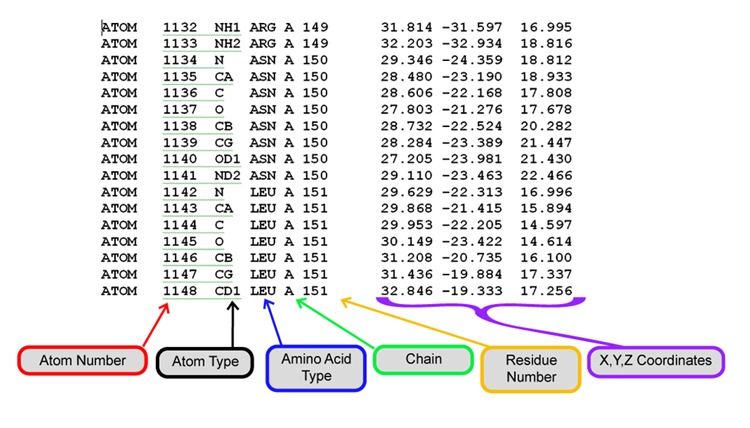
\includegraphics[scale=0.65]{images/pdbFile.jpg}
	\caption{Formato PDB. Fonte\cite{pdbFormat}}
	\label{fig:pdb-format}
\end{figure}

Un file PDB è essenzialmente un contenitore di coordinate X, Y, Z per ogni atomo di una struttura molecolare. I programmi di visualizzazione molecolare traducono queste coordinate X, Y, Z in immagini tridimensionali interattive. La maggior parte dei file PDB inizia con informazioni scritte sulla struttura, il laboratorio che l'ha determinata e le tecniche utilizzate nel laboratorio. Eventuali commenti come questi iniziano sempre con la parola "REMARK" e verranno ignorati dai software di visualizzazione. Esiste anche una versione XML del formato PDB chiamata PDBML.

\par Il formato originale (PDB) è però limitato dalla larghezza delle schede perforate per computer a 80 caratteri per riga. Intorno al 1996, il formato mmCIF (macromolecular Crystallographic Information file), un'estensione del formato CIF, è stato gradualmente introdotto. mmCIF è diventato il formato standard per l'archivio PDB nel 2014 e nel 2019, il wwPDB ha annunciato che le deposizioni per i metodi cristallografici sarebbero state accettate solo in formato mmCIF.

\subsubsection{Database di proteine}

Il \textit{Protein Data Bank }(PDB) è un archivio di strutture tridimensionali di macromolecole biologiche determinate sperimentalmente. È il deposito principale dei centri biologici di struttura. I dati contenuti nell'archivio includono coordinate atomiche, fattori di struttura cristallografici e dati sperimentali NMR. Oltre alle coordinate, ogni deposizione include anche i nomi delle molecole, le informazioni sulla struttura primaria e secondaria, i riferimenti al database di sequenze, ove appropriato, e le informazioni sull'assemblaggio biologico e sul ligando, i dettagli sulla raccolta dei dati e sulla soluzione della struttura e le citazioni bibliografiche. 

\par Quando il PDB fu fondato, nel 1971, conteneva appena 7 strutture proteiche ed era frutto di una congiunzione fra il Cambridge Crystallographic Data Centre (UK)e il Brookhaven National Laboratory (USA), e da allora si è reso protagonista di una crescita pressoché esponenziale nel numero di strutture, che non mostra alcun segno di rallentamento. Nel 1998 il PDB è stato trasferito al Research Collaboratory for Structural Bioinformatics (RCSB). Nel 2003, con la formazione del \textit{wwPDB}, il PDB è diventato un'organizzazione internazionale.  I membri fondatori sono PDBe (Europa), RCSB (USA) e PDBj (Giappone). Il BMRB (Biological Magnetic Resonance Data Bank) si è unito nel 2006. Ciascuno dei quattro membri di wwPDB può fungere da centro di deposito, elaborazione dati e distribuzione dei dati PDB.  Il trattamento dei dati si riferisce al fatto che il personale del wwPDB esamina e annota ogni voce presentata. I dati vengono quindi automaticamente verificati per verificarne la plausibilità.\\

\par \textit{UniProt} (Universal Protein Resource) è il più grande database bioinformatico per le sequenze proteiche di tutti gli organismi viventi e dei virus. Molte informazioni derivano da progetti di sequenziamento del genoma. I database UniProt sono UniProt Knowledgebase (UniProtKB), UniProt Reference Cluster (UniRef) e UniProt Archive (UniParc). Il consorzio UniProt e le istituzioni ospitanti EMBL-EBI, SIB (Swiss Institute of Bioinformatics) e PIR (Protein Information Resource) sono impegnati nella conservazione a lungo termine dei database UniProt.

\begin{figure}[!htb]
	\centering
	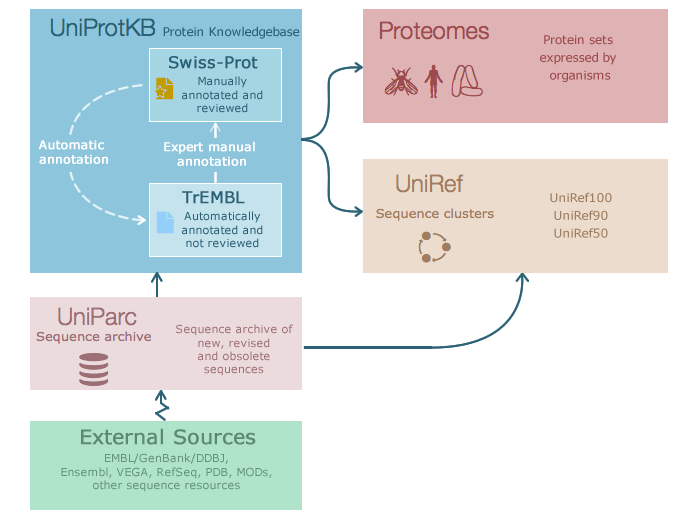
\includegraphics[scale=0.5]{images/uniprot.png}
	\caption{Struttura di UniProt. Fonte\cite{uniProt}}
	\label{fig:uniprot}
\end{figure}

EMBL-EBI e SIB insieme mantenevano Swiss-Prot e TrEMBL, mentre PIR produceva il Protein Sequence Database (PIR-PSD). Questi due set di dati coesistevano con diverse priorità di copertura e annotazione della sequenza proteica.  TrEMBL (Translated EMBL Nucleotide Sequence Data Library) è stato originariamente creato perché i dati di sequenza venivano generati a un ritmo che superava la capacità di Swiss-Prot di tenere il passo.  Nel frattempo, PIR ha mantenuto il PIR-PSD e i relativi database, incluso iProClass, un database di sequenze proteiche e famiglie curate.  Nel 2002 i tre istituti hanno deciso di unire le proprie risorse e competenze e hanno costituito il consorzio UniProt.\\

\par EMBL (European Molecular Biology Laboratory) è un'organizzazione di ricerca intergovernativa finanziata da oltre 20 Stati membri, potenziali e associati. L'istituto europeo di bioinformatica, EMBL-EBI (EMBL-European Bioinformatics Institute) si trova a Cambridge e gestisce, insieme all'NCBI (National Center for Biotechnology Information, USA), i maggiori database di sequenze nucleotidiche e proteiche. Uno dei ruoli dell'EMBL-EBI è quello di indicizzare e mantenere i dati biologici in una serie di database, inclusi Ensembl (che ospita i dati della sequenza di interi genomi), UniProt e PDB. Fornisce anche una varietà di servizi e strumenti online, come BLAST o lo strumento di allineamento di sequenze Clustal$\Omega$.\\

\par EMDB (Electron Microscopy Data Bank) è una banca dati di microscopia elettronica (EMDB). È un archivio pubblico per mappe volumetriche di crio-microscopia elettronica e tomografia di complessi macromolecolari e strutture subcellulari. Copre una varietà di tecniche, tra cui l'analisi di singole particelle, la tomografia elettronica e la cristallografia elettronica. È stato fondato nel 2002 dall'EMBL-EBI e nel gennaio 2021 è divenuto un archivio gestito dalla wwPDB. \\

\par La predizione della struttura è importante per un semplice motivo: i biochimici conoscono oggi la sequenza amminoacidica per più di 225 milioni di proteine\supercite{proteienDBentries} (UniProt, con circa 4.5-5 milioni aggiunte ogni mese) ma sono state determinate solamente circa 160 000 strutture tridimensionali di proteine\supercite{proteienDBentries} (PDB\footnote{In particolare è da notare che spesso sono presenti più strutture per una data proteina, infatti le strutture proteiche distinte determinate sono circa 55 000. Al 3 Febbraio 2022 sono presenti 162 913 strutture di proteine nella versione dell'RCSB. Nel PDB ci sono anche strutture di altre macromolecole (complessi di acidi proteici-nucleici, DNA e RNA) per un totale, incluse le proteine, di 186 670\supercite{pdbStats}. Nel wwPDB (database globale) vi sono in totale 197 961 strutture di macromolecole\supercite{wwpdbStats}.}, con poco più di 10 000 strutture aggiunte ogni anno). 

\begin{figure}[!htb]
	\centering
	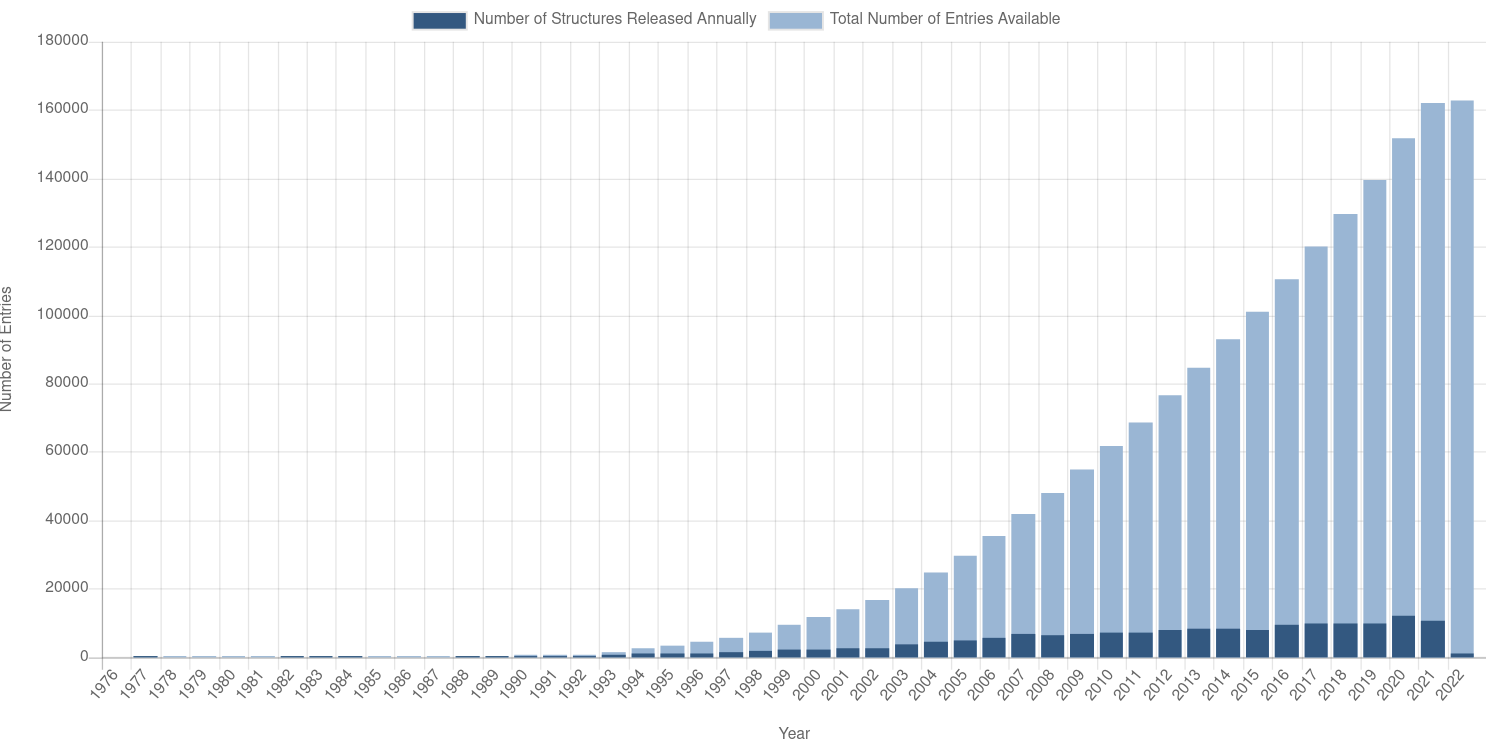
\includegraphics[scale=0.3]{images/pdb-statistica.png}
	\caption{Crescita complessiva del numero di strutture di proteine pubblicate nel PDB. Fonte\cite{pdbStats}}
	\label{fig:pdb-statistica}
\end{figure}


\par Sono disponibili anche database di modelli 3D di strutture proteiche, come ModBase. Un database di questo tipo è stato fondato dall'EMBL-EBI in congiunzione con DeepMind grazie al successo di AlphaFold: \textit{AlphaFold DB}.

\par AlphaFold DB è un database apertamente accessibile di previsioni ad alta precisione di strutture proteiche. Basato su AlphaFold v2.0, ha consentito un'espansione senza precedenti della copertura strutturale dello spazio noto della sequenza proteica. AlphaFold DB fornisce l'accesso programmatico e la visualizzazione interattiva delle coordinate atomiche previste di una proteina, e le relative misure di confidenza stimate. La versione iniziale di AlphaFold DB contiene oltre 360 000 strutture predette in 21 proteomi di organismi modello. Il database sarà presto ampliato per coprire la maggior parte delle sequenze rappresentative del set di dati UniRef90 (oltre 100 milioni)\supercite{varadi2021alphafold}.

\par Nella prima versione di AlphaFold DB si è tentato di prevedere la maggior parte delle sequenze nel proteoma di riferimento UniProt nell'intervallo di lunghezza di (16, 2 700) amminoacidi (oltre a frammenti di 1 400 residui per coprire proteine umane più lunghe) per gli organismi attualmente coperti. Sono state escluse le sequenze che contengono amminoacidi non standard. Non vengono fornite isoforme multiple.

\par AlphaFold DB archivia e fornisce accesso alle coordinate atomiche nei formati PDB e mmCIF, mentre fornisce il PAE (Predicted Aligned Error) in JSON.



\subsection{Rappresentazione grafica}

I file di struttura possono essere visualizzati tramite una rappresentazione grafica tridimensionale utilizzando uno dei numerosi software disponibili\footnote{Una lista più completa di software grafici per macromolecole è consultabile al seguente link (RCSB): https://www.rcsb.org/docs/additional-resources/molecular-graphics-software.}, inclusi:

\begin{figure}[!htb]
	\centering
	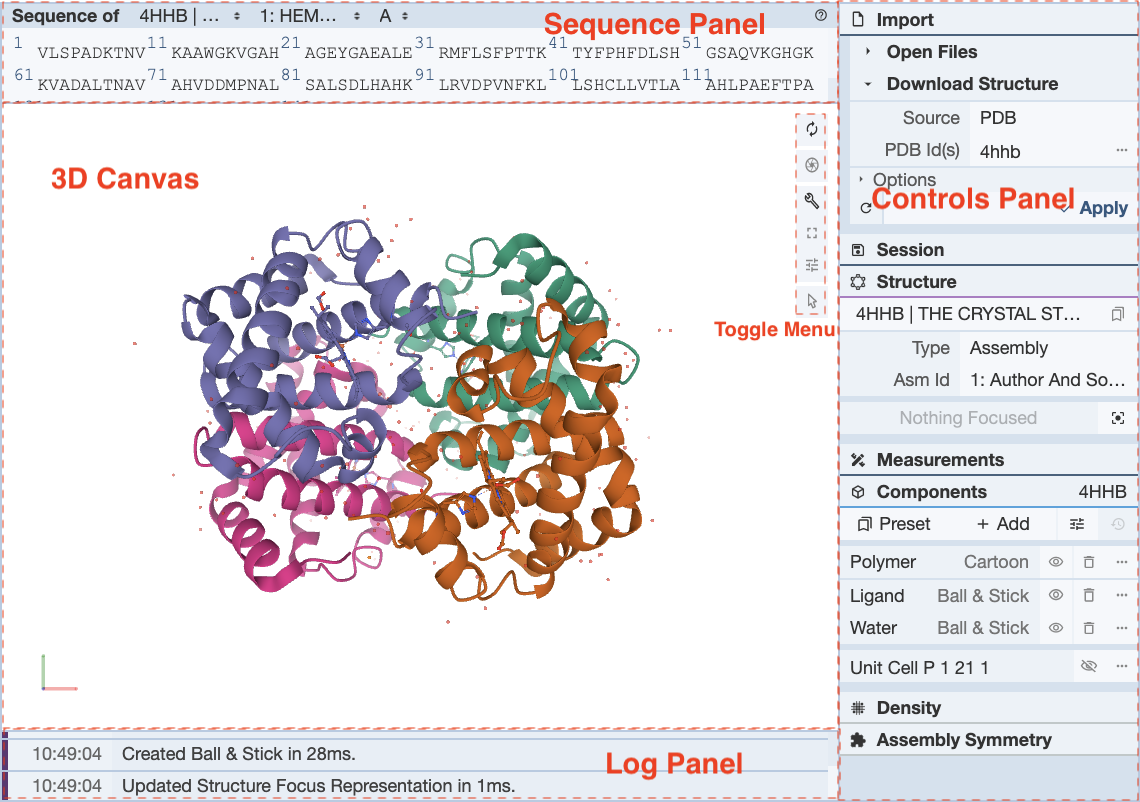
\includegraphics[scale=0.7]{images/molstar.png}
	\caption{Interfaccia utente di Mol* utilizzata nel sito del PDB. Fonte\cite{pdbStats}}
	\label{fig:ui-molstar}
\end{figure}

\begin{itemize}
	\item Mol*, frutto di una collaborazione aperta avviata da PDBe e RCSB PDB per fornire uno stack tecnologico di strumenti di analisi di macromolecole; è usato sul sito del PDB ed è possibile anche caricare i propri file
	\item Jmol, software open-source scritto in Java 
	\item PyMOL
	\item QuteMol, sviluppato anche da Paolo Cignoni (ISTI-CNR)
	\item Chimera
	\item RasMol
\end{itemize}

\subsubsection{Tipi di rappresentazioni grafiche}

I principali tipi di rappresentazione grafica sono: 

\begin{figure}[!htb]
	\centering
	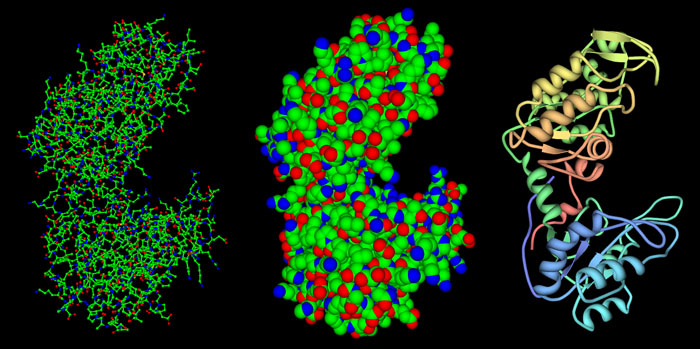
\includegraphics[scale=0.6]{images/rappresentazioni.jpg}
	\caption{Da sinistra a destra, rappresentazioni: wire-frame, space-fill, ribbon. Fonte\cite{pdbStats}}
	\label{fig:rappresentaizoni}
\end{figure}

\begin{itemize}
	\item \textit{ribbon}, viene mostrata solo la backbone della proteina, rappresentata come un nastro che contiene tutti gli atomi (in realtà spesso solamente gli atomi $C_{\alpha}$). Mette in luce sia il ripiegamento che le strutture secondarie della proteina; è una delle rappresentazioni più utilizzate\\
	
	\item \textit{wire-frame}, vengono rappresentati solo i legami covalenti tra gli atomi, tracciando una linea per ciascuno dei legami. In molti casi viene utilizzata la rappresentazione \textit{ball-and-stick} (asta e sfera) per rendere più facile la comprensione della forma tridimensionale. Rivela la connettività degli atomi nella proteina ma può sommergere il ricercato con una quantità eccessiva di dettagli\\

	\item \textit{space-fill}, gli atomi vengono mostrati come sfere, la cui grandezza è spesso relativa al loro raggio di van der Waals. La rappresentazione è chiara e colorata, fornisce la forma generale della proteina ma non fornisce altre informazioni aggiuntive, perciò viene raramente usata nel contesto scientifico\\

	\item \textit{surface}, utile per interpretare l'interazione della proteina con l'ambiente esterno
\end{itemize}

Ogni approccio mette in risalto informazioni differenti, e una rappresentazione combinata può risultare spesso la scelta vincente per mostrare più dettagli in una singola immagine.

\par È possibile anche colorare la rappresentazione sulla base di determinate caratteristiche, come il potenziale elettrostatico, la conservazione evolutiva, il grado di flessibilità della catena o l'appartenenza a una delle possibili catene polipeptidiche. Ad esempio la rappresentazione della superficie colorata in base al potenziale elettrostatico è di aiuto ai ricercatori nella scoperta di siti di legame della proteina.

\begin{figure}[!htb]
	\minipage{0.6\textwidth}
	\centering
	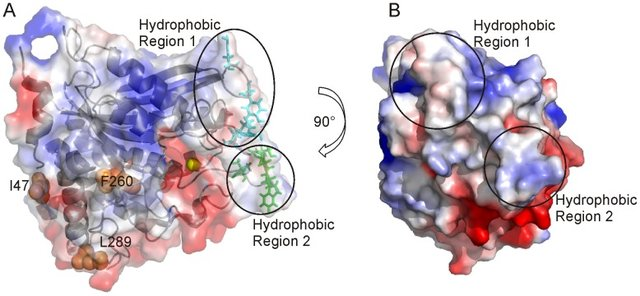
\includegraphics[scale=2]{images/combinata-ecc.jpg}
	\caption{(A) rappresentazione combinata; è presente sia la rappresentazione della superficie che ribbon che ball-and-stick. (B) rappresentazione della superficie colorata in base al potenziale elettrostatico (i potenziali negativi sono rossi, quelli potenziali positivi blu e i potenziali neutri bianchi). Fonte: \cite{castaldo2013soluble}}
	\label{fig:rappresentazione-combinata}
	\endminipage\hfill
	\minipage{0.38\textwidth}
	\centering
	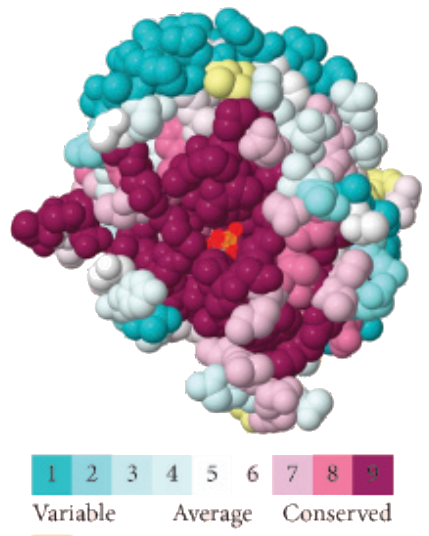
\includegraphics[scale=0.35]{images/conservazione.png}
	\caption{Rappresentazione space-fill colorata in base alla conservazione evolutiva. Fonte \cite{kessel_ben-tal_2018}}
	\label{fig:rappresentazione-evolutiva}
	\endminipage\hfill
\end{figure}

\subsection{CASP ed excursus storico}  \label{sec:CASP}

Dal 1994 il campo del PSP è stato stimolato, monitorato e quantitativamente valutato dalla competizione biennale CASP (\textit{Critical Assessment of Structure Predictions}). CASP è una sfida nella quale gruppi di ricerca si sfidano cercando di realizzare predizioni di strutture di proteine. È nota la sequenza amminoacidica di queste proteine target ma non la struttura sperimentale. Queste sequenze di proteine provengono da laboratori  congiunti: è pianificata la determinazione delle loro strutture native in vitro, che verrà infine utilizzata per stabilire l'accuratezza dei metodi in gara.

\par Questi esperimenti a livello di comunità sono cresciuti significativamente nel corso delle edizioni: dai 33 target e i 100 modelli sottomessi nel 1994 (CASP1) agli 82 target e più di 55 000 modelli sottomessi nel 2018 (CASP13)\supercite{abbass2020enhancing}.

\par Ogni due anni un insieme di sequenze di proteine sono rilasciate gradualmente nel corso di un paio di mesi, durante i quali gruppi di ricerca da tutto il mondo tentano di predire le loro strutture 3D e inviano i loro modelli (fino a 5 per target).

\par Nei primi 6 round (CASP1-6), i target erano classificati in 3 categorie: \textit{comparative modeling}, \textit{fold recognition} e \textit{ab initio}. Da allora i target sono stati classificati solo in 2 classi: le famose \textit{template-based modeling} e \textit{template-free modeling}. I target nella categoria TBM sono considerati "facili" mentre quelli in FM sono considerati difficili. È presenta anche la divisione fra metodi completamente automatici e previsioni ottenute usando intervento umano.

\par È interessante notare che nei primi round del CASP, la previsione della struttura secondaria era una categoria separata. Questa categoria è stata cancellata dopo che gli organizzatori hanno notato che i vincitori di tale categoria utilizzavano un approccio circolare: prevedevano la struttura 3D e utilizzavano la struttura del modello per decifrare gli elementi della struttura secondaria.

\par I risultati sono valutati sulla base di vari criteri, come il numero di residui la cui posizione è stata predetta con un certo livello di accuratezza, identificazione di strutture secondarie, limiti dei domini, contatti fra residui, regioni disordinate, ecc.

\par Analizzando i risultati del CASP negli anni si può notare che i metodi basati su un approccio fisico, nonostante l'aumento della potenza computazionale, hanno subito solo lievi miglioramenti.

\par L'importanza del CASP per la biologia strutturale è alta anche per il contributo che ha dato alla creazione dei metodi automatici, accessibili anche ai non esperti.


\subsubsection{Excursus storico}

Dal punto di vista biologico e sperimentale sulle proteine, tra i punti di riferimento più importanti ci sono\supercite{alberts2018essential}:
\begin{itemize}
	\item nel 1838 è stato proposto il nome \textit{proteina}
	\item durante il XIX secolo vengono scoperti la maggior parte dei 20 amminoacidi 
	\item nel 1864 è stata cristallizzata e denominata l'emoglobina
	\item nel 1894, come già citato, Fischer ha proposto l'analogia chiave-lucchetto per le interazioni fra enzimi e substrato
	\item nel 1897 vengono gettate le basi per l'enzimologia
	\item nel 1926 viene dimostrato che le proteine possono essere enzimi e viene sviluppata l'ultracentrifugazione, usata per stimare il peso molecolare dell'emoglobina
	\item negli anni '30 vengono proposte le prime teorie sulla denaturazione delle proteine
	\item nel 1933 viene introdotta l'elettroforesi
	\item nel 1934 viene mostrata la prima diffrazione a raggi-X di una proteina
	\item nel 1942 viene sviluppata la cromatografia
	\item nel 1951 vengono proposte le strutture secondarie $\alpha$-eliche e foglietti-$\beta$
	\item nel 1955 viene sequenziata la prima proteina (insulina)
	\item nel 1956 viene prodotta la prima "impronta digitale" di una proteina, mostrando la causa dell'anemia falciforme
	\item nel 1960 viene descritta la prima struttura tridimensionale tramite cristallografia a raggi-X a risoluzione di 2 \angstrom
	\item nel 1966 viene descritta la struttura tridimensionale del lisozima, il primo enzima ad essere analizzato a risoluzione atomica
	\item nel 1975 Henderson e Unwin determinano la prima struttura 3D di una proteina di membrana usando una ricostruzione al computer da micrografie elettroniche
	\item nel 1983 viene usato la spettroscopia NMR per determinare la struttura 3D di una proteina
	\item nel 1988 vengono sviluppati metodi per l'uso della spettrometria di massa nell'analisi di proteine e altre macromolecole
	\item nel 2003 è stato completato il progetta genoma umano
	\item tra il 1996-2013 vengono rifiniti i metodi nell'uso della spettrometria di massa per identificare proteine in miscugli complessi
	\item tra il 1975-2013 Henderson e altri rifiniscono i metodi nell'utilizzo della cryo-EM per la determinazione della struttura di larghi complessi proteici a risoluzione atomica
\end{itemize}

I primi passi della \textit{bioinformatica }risiedono nei primi anni '60, quando ancora i desktop computer erano solo un'ipotesi e il DNA non poteva essere sequenziato. Questi passi andavano in direzione di metodi computazionali per l'analisi della sequenza delle proteine. Margaret Dayhoff è considerata la madre della bioinformatica: ha infatti sviluppato il primo software bioinformatico (COMPROTEIN) e il primo database per le sequenze biologiche (\textit{Atlas of Protein Sequence and Structure}, contenente 65 sequenze di proteine). Il codice a una lettera per gli amminoacidi si deve sempre alla Dayhoff\supercite{gauthier2019brief}. 

\par È in questi anni che è stato sviluppato il primo modello di sostituzione degli amminoacidi per la filogenetica. Anche l'approccio \textit{ab initio} (non per le proteine) è emerso negli anni '60 a partire dal campo della chimica computazionale, grazie principalmente a Warshel, Levitt, Karplus\footnote{Nel 2013 il premio Nobel per la chimica è stato assegnato proprio a questi scienziati che hanno contribuito sin da quegli anni al campo della biofisica molecolare computazionale.}. Il primo programma per calcolare l'energia potenziale nelle proteine è stato sviluppato nel 1969 da Lifson e Levitt\supercite{levitt1969refinement}.

\par Le predizioni di strutture basate sui metodi \textit{ab initio} sono emerse nella metà degli anni '80, prima per piccoli peptidi e poi per polipeptidi. La prima simulazione di MD su una proteina è stata realizzata nel 1977 da McCammon, Gelin e Karplus\supercite{mccammon1977dynamics}, studiando la dinamica di ripiegamento di una proteina di 58 amminoacidi rappresentata esplicitamente ma simulata nel vuoto. Questo studio seguì il lavoro pionieristico di Levitt e Warshel del 1975 (\textit{Computer simulation of protein folding}\supercite{levitt1975computer}) sulla stessa proteina che era però rappresentata in modo più semplicistico: ogni amminoacido era rappresentato da due sfere. 

\par Intorno all'inizio degli anni '90 è emerso dalla biologia il campo della bioinformatica, sulla base dall'analisi delle proteine, come dimostra anche l'instaurazione del CASP.

\par Nel 2007 si è raggiunta un'accuratezza nella predizione della struttura di proteine (a singolo dominio con massimo 90 residui) tra i 2 e i 6 \angstrom    $\,$(modellazione per omologia)\supercite{dill2008protein}.

\par Nel 2020 AlphaFold è stato reputato vincitore del CASP riuscendo praticamente a risolvere il problema del PSP (per determinate categorie di proteine). 


\section{Annotazioni 1D sulla struttura} \label{sec:predizione-structural-features}
%- praveen 2014
%- pal 

Le "annotazioni monodimensionali sulla struttura delle proteine" (1D PSA) sono astrazioni che descrivono la disposizione della backbone proteica. 

\begin{figure}[!htb]
	\centering
	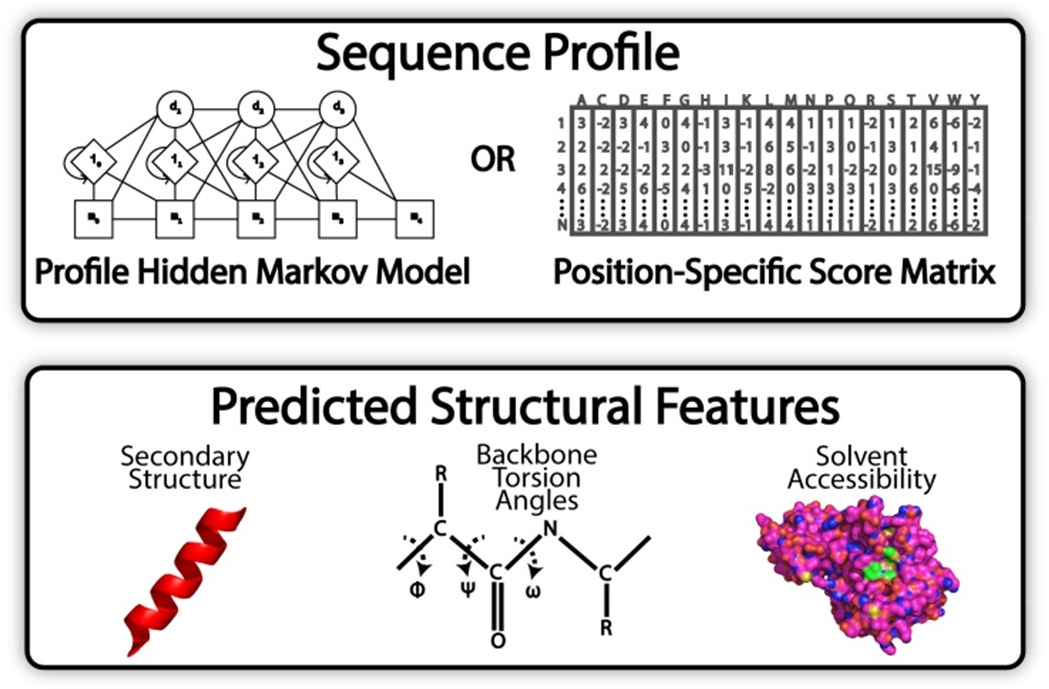
\includegraphics[scale=1.5]{images/1dpsa.png}
	\caption{Annotazioni 1D nella pipeline generica di un metodo odierno per il PSP. Fonte\cite{pearce2021deep}}
	\label{fig:1dpsa}
\end{figure}

Le annotazioni monodimensionali delle sequenze possono essere legate a due tipi di proprietà:
\begin{itemize}
	\item proprietà esplicitamente correlate con la struttura degli amminoacidi
	\item proprietà statistiche
\end{itemize}

Annotazioni del 1° tipo sono collegate a: formazione di determinate strutture secondarie, esposizione al solvente circostante (\textit{solvent accessibility}), determinati angoli di torsione, interazioni con alcuni amminoacidi, ecc. (es. GenTHREADER, SPARKS-X).

\par Le proprietà statistiche vengono invece identificate tramite le frequenze degli amminoacidi in vari MSA. Un modo di rappresentare queste tendenze è tramite \textit{profili}, i quali denotano amminoacidi che frequentemente appaiono in certe posizioni dell'allineamento. Un profilo del genere è più informativo di una semplice sequenza amminoacidica: contiene informazioni evolutive (es. livelli di conservazione di specifiche posizioni nella sequenza). Il profilamento della sequenza avviene tipicamente tramite HMM (Hidden Markov Model) o PSSM (Position-specific score matrix).

\par Dato che tutti gli step successivi, in ogni caso (compresi metodi end-to-end), dipendono dalla qualità dell'MSA, la generazione di allineamenti di alta qualità è di incredibile importanza per il PSP. A prescindere dall'approccio e dall'utilizzo o meno del DL, sfruttare le informazioni evolutive è risultato essere lo step più importante.

\subsection{Allineamento di sequenze} \label{sec:MSA}
{
	Un allineamento di sequenze multiple (MSA) è una disposizione di più di due sequenze di amminoacidi o nucleotidi allineate in modo da posizionare i residui delle diverse sequenze in colonne verticali in una maniera appropriata. I metodi di MSA sono utilizzati per l'analisi del proteoma e del genoma; sono il passo iniziale essenziale nella maggior parte dei confronti filogenetici. Sono ampiamente utilizzati per aiutare a ricercare caratteristiche comuni nelle sequenze e possono essere usati per aiutare a prevedere le strutture bi e tridimensionali di proteine e acidi nucleici. Un MSA, in essenza, mostra il grado di similarità evolutiva tra le sequenze. 
	
	\par In genere si assume che le sequenze che si vuole allineare siano filogeneticamente correlate e, quindi, omologhe. In questo caso, l'allineamento ideale avrà residui omologhi allineati nelle colonne.
	
	\begin{figure}[!htb]
		\centering
		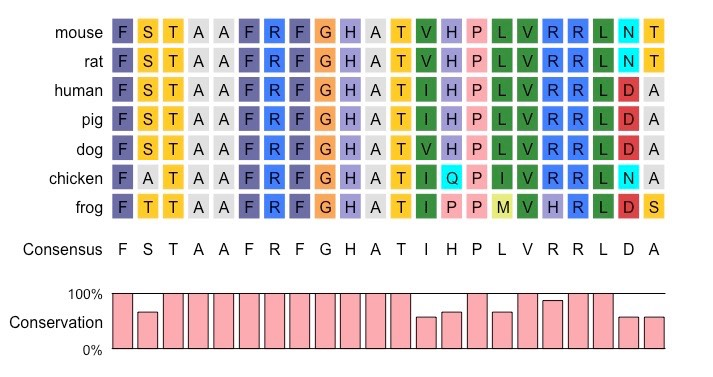
\includegraphics[scale=0.5]{images/msa.jpeg}
		\caption{Multiple sequence alignment schematica di una sequenza proteica di varie specie. Fonte\cite{msaBioNinja}}
		\label{fig:msa}
	\end{figure}
	
	\par Le sequenze di proteine in genere risultano avere un grado di somiglianza maggiore rispetto alle sequenze nucleotidiche. Ciò è dovuto alla degenerazione del codice genetico e al fatto che quasi per ogni amminoacido esistono vari codoni che lo codificano, perciò differenti sequenze nucleotidiche possono codificare esattamente la stessa sequenze di amminoacidi.
	
	\par Un allineamento di sequenze multiple (MSA) può essere utilizzato per tracciare l'entità della divergenza evolutiva tra sequenze correlate. Rispetto a una singola sequenza, l'MSA fornisce informazioni sulle tendenze evolutive degli amminoacidi in ciascuna posizione della sequenza, il che aiuta a caratterizzare un "profilo" della sequenza.
	
	\par Un modo per generare un MSA è cercare grandi data set di sequenze proteiche e allinearli alla sequenza target. All'interno di un metodo per generare un MSA vengono utilizzati vari metodi per massimizzare i punteggi e la correttezza degli allineamenti.  Ogni metodo utilizza un'euristica che cerca di replicare il processo evolutivo e ottenere un allineamento realistico.	Ci sono vari tool per creare MSA, ad esempio: Clustal$\Omega$, MAFFT, MUSCLE, T-Coffee.
}

\section{Annotazioni 2D sulla struttura}

Le annotazioni bidimensionali sulla struttura delle proteine (2D PSA) permettono di ricavare restrizioni spaziali come contatti inter-residuo a lunga distanza, distanze specifiche o legami idrogeno. 

\begin{figure}[!htb]
	\centering
	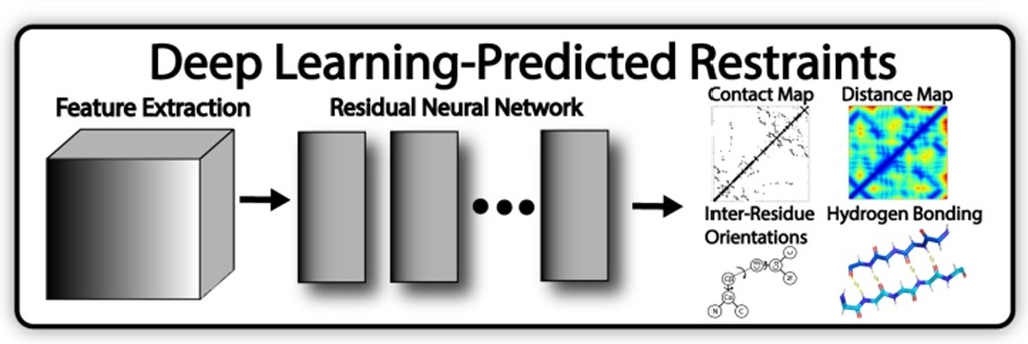
\includegraphics[scale=1.5]{images/2dpsa.png}
	\caption{Annotazioni 2D nella pipeline generica di un metodo odierno per il PSP. Fonte\cite{pearce2021deep}}
	\label{fig:2dpsa}
\end{figure}

Le annotazioni si basano sulla predizione dei contatti fra i residui sulla base, ad esempio, di informazioni co-evolutive (\textit{correlated mutation}), generando o una \textit{contact map}, o un \textit{distogramma} o una \textit{distance map}. 

\begin{figure}[!htb]
	\centering
	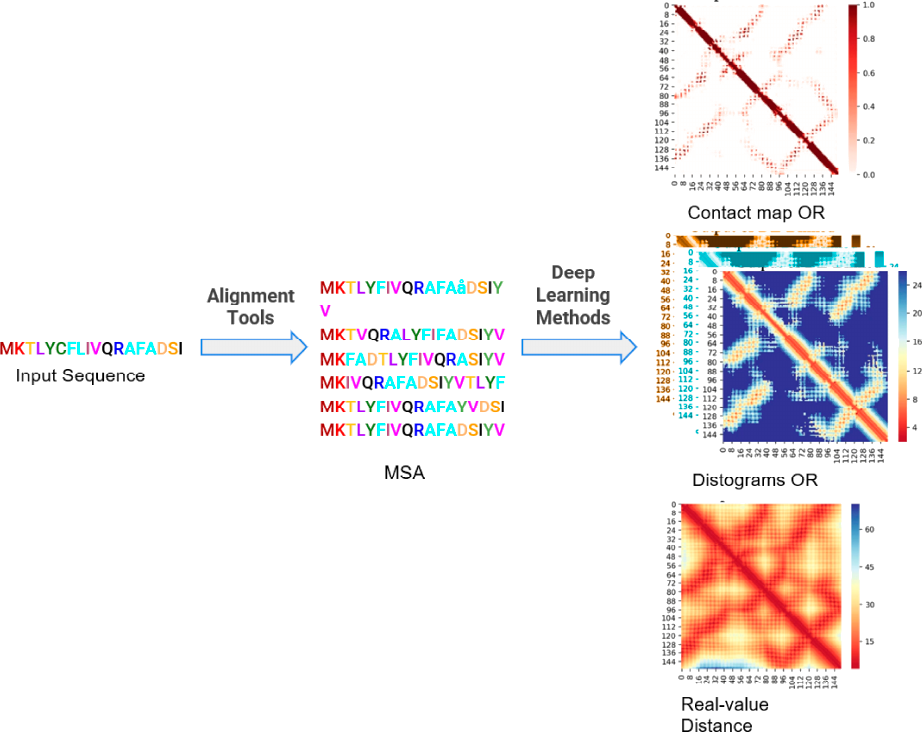
\includegraphics[scale=0.6]{images/FM-template.png}
	\caption{Schema generali di contact prediction basata su DL. Fonte\cite{pakhrin2021deep}}
	\label{fig:fm-template-dl}
\end{figure}

\par I progressi nella previsione dei contatti sono rimasti stagnanti per qualche tempo. Tuttavia, si è verificato un balzo nell'accuratezza della previsione dei contatti quando gli algoritmi hanno iniziato a utilizzare approcci di previsione globale. I primi metodi prevedevano principalmente i contatti tra le coppie di residui uno alla volta utilizzando tecniche come l'informazione reciproca, ignorando così le interazioni con altre coppie di residui e il contesto globale in cui si verificavano le interazioni; questo è in gran parte il motivo per cui era difficile per questi metodi locali distinguere tra interazioni dirette e indirette. L'introduzione di modelli statistici globali determinati attraverso l'uso dell'analisi di accoppiamento diretto (DCA) è stata in grado di distinguere con maggiore successo tra queste interazioni dirette e indirette. Il DL ha successivamente rivoluzionato il campo della predizione dei contatti sin dal suo debutto nel CASP10, facendo progredire negli ultimi questo campo dalla predizione binaria dei contatti alla predizione della distanza a valori reali o probabilistica (distogrammi); spesso vengono utilizzate delle \textit{deep residual neural network} (\textit{ResNet}).  

\par Data la natura \textit{black-box} dei metodi di DL è stata ad esempio proposta InterPretContactMap che fa riferimento al campo della xAI (explainable AI); combina reti neurali profonde con meccanismi di attenzione per aumentare la comprensibilità della predizione dei contatti. \\

È dal CASP11 che la predizione di una \textit{contact map} è diventata una chiave fondamentale della pipeline dei metodi per il PSP. La predizione dei contatti può essere classificata in due categorie:

\begin{itemize}
	\item correlated-mutation-based
	\item ML-based
\end{itemize}

Le \textit{contact map} (descritte nella sez. \ref{sec:modelli-output}) possono essere divise in 4 categorie a seconda di quanto siano lontani fra loro i residui nella sequenza:

\begin{enumerate}
	\item local, <6 residui
	\item short-range, 6-11 residui
	\item medium-range, 12-23 residui
	\item long-range, >24 residui
\end{enumerate}

I contatti locali descrivono in realtà le strutture secondarie, pertanto i contatti che risultano essere più utili sono quelli a medio e lungo raggio.

\subsection{\textit{correlated mutation}}
{
	L'apparizione di mutazioni nelle sequenze delle proteine durante la loro evoluzione dipende da aspetti sia strutturali che funzionali. È interessante notare come l'analisi delle sequenze di famiglie di proteine mostri che certe posizioni tendono a \textit{coevolvere}. In altre parole l'apparizione di una mutazione in una posizione è accompagnata da una mutazione in un'altra posizione. 
	
	\par È stato suggerito che un tale collegamento possa avvenire in posizioni vicine nello spazio tridimensionale e che i residui considerati interagiscano fra loro. Se una mutazione in una posizione porta a una distruzione della sua interazione con la posizione adiacente, una mutazione compensatoria di quest'ultima potrebbe rimediare al problema.
	
	\par Ad esempio, se due posizioni erano originariamente polari e coinvolte in un'interazione elettrostatica favorevole, la mutazione di una posizione da polare a non polare distruggerebbe l'interazione. Se però la posizione adiacente muta anch'essa da polare a non polare, l'interazione originale può tramutarsi in un'altra interazione favorevole, stavolta non polare.
	
	\par Ciò suggerisce che sia possibile inferire posizioni a contatto nella struttura ripiegata di una proteina analizzandone le variazioni nella sequenza attraverso la sua evoluzione e osservando quali posizioni sono \textit{coevolute}. Gli accoppiamenti evoluzionisticamente inferiti possono essere usati come vincoli durante la modellazione.
	
	\begin{figure}[!htb]
		\centering
		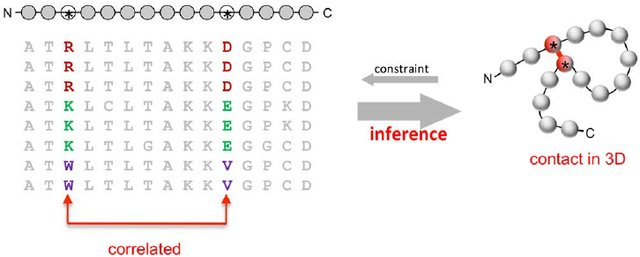
\includegraphics[scale=0.65]{images/correlated-mutation.jpg}
		\caption{In alto, sequenza della proteina da predire, in cui ogni amminoacido è un cerchio. Sotto, un MSA con le sequenze di una famiglia correlata, tutte con lo stesso ripiegamento. A destra l'inferenza del contatto delle posizioni coevolute. Fonte\cite{marks2011protein}}
		\label{fig:correlated-mutation}
	\end{figure}
	
	\par Ci sono 3 principali ostacoli a questo approccio: rumore statistico (molte correlazioni sono solo frutto di rumore e quindi insignificanti), correlazioni fra residui distanti e numero insufficiente di posizioni correlate. Il metodo non risulta applicabile quando ci sono poche sequenze omologhe. Nonostante l'idea non sia nuova, solo nell'ultimo decennio tali metodi sono divenuti abbastanza accurati da poter essere usati nel PSP; metodi noti sono EVfold, Rosetta-GREMLIN, FILM3, MetaPSICOV, ecc.
	
}

\subsection{\textit{contact prediction ML-based}}

La predizione di contatti tra i residui è stata ampiamente utilizzata per oltre un decennio nel campo del PSP. Tuttavia, recentemente, il paradigma si è spostato verso la previsione della probabilità di intervalli di distanza, noti anche come \textit{distogrammi} (distanza + istogramma). 

\par Per una sequenza di lunghezza $L$, un distogramma è una matrice $L \times L$, che mostra l'istogramma delle distanze tra coppie. I distogrammi sono matrici simmetriche rispetto alla diagonale. Ogni "pixel" sulla mappa rappresenta una distanza tra una coppia di residui nella sequenza. Le distanze in un distogramma sono relative, il che significa che le distanze tra i residui sono invarianti rispetto alle rotazioni e alle traslazioni 3D.

\par Le distanze sono \textit{binned}\footnote{Ciò vuol dire che i valori dei dati originali che rientrano in un dato piccolo intervallo, un \textit{bin}, sono sostituiti da un valore rappresentativo di quell'intervallo, spesso il valore centrale.  È una forma di quantizzazione.}, pertanto il distogramma può avere tanti canali quanti sono i \textit{bin}, ovvero $L\times L \times bins$ tensori\footnote{In matematica, la nozione di tensore generalizza tutte le strutture definite usualmente in algebra lineare a partire da un singolo spazio vettoriale.}.  \\

\par La previsione della distanza tra i residui proteici è la previsione di una matrice (2D) di distanze tra coppie a partire da una sequenza proteica (1D). Tale problema può essere confrontato con quello della stima della profondità monoculare in \textit{computer vision} (vedi fig. \ref{fig:distogramma-cane}).

\par Nell'\textit{image depth prediction}, viene fornita una matrice dell'immagine come input e viene prevista come output una matrice di profondità in cui ogni pixel ha una profondità prevista (distanza dalla fotocamera all'oggetto). Similmente al problema della previsione della profondità, la previsione della distanza nel PSP prende in input un volume tridimensionale (altezza × larghezza × canali, tensore 3D) e genera una mappa della distanza con la stessa dimensione dell'input (altezza × larghezza) ma con un singolo canale. 

\par Tuttavia, i canali di input nei problemi di visione artificiale vanno da uno a tre (i canali RGB o HSV), ma possono arrivare alle centinaia di canali nel PSP, a seconda delle caratteristiche di input.

\begin{figure}[!htb]
	\centering
	\includegraphics[scale=0.1]{images/distogramma.png}
	\caption{Confronto fra "image depth prediction" e "distance prediction". Fonte\cite{pakhrin2021deep}}
	\label{fig:distogramma-cane}
\end{figure}

\par Fino al CASP13 i tentativi di predire dei distogrammi erano stati poco efficaci, è solo con il metodo di Xu, trRosetta e AlphaFold1 che tale tecnica è maturata. La tecnica di DL principalmente utilizzata è l'uso di ResNet.

\par Il metodo di Xu, implementato in Raptor X, discretizza le distanze di interazione $C_{\beta}$-$C_{\beta}$ in 25 intervalli (compresi fra $4.5\, \angstrom$ e $16\, \angstrom$). È possibile ottenere una \textit{contact map} da questa \textit{distance map} sommando tutti valori di probabilità previsti corrispondenti a distanze $\leq 8$ $\angstrom$\supercite{pakhrin2021deep}. \\

\par La predizione delle distanze a valori reali è un task ancora più difficile. Consiste nel predire le esatte distanze fisiche sull'intera \textit{distance map} accuratamente. I metodi odierni utilizzano ResNet o GAN o meccanismi di attenzione; degli esempi sono PDNET e RealDist.

\section{Predizione della struttura 3D}

\subsection{\textit{homology modeling}}
{
	Nella modellazione per omologia ci si affida a somiglianze nella sequenza tra la proteina target e i template. I metodi per omologia sono perciò basati sul paradigma: \\
	\say{\textit{la sequenza codifica per la struttura}}.
	Due proteine si definiscono \textit{omologhe} quando hanno un progenitore comune nella loro storia evolutiva; una notevole somiglianza fra due sequenze è una forte evidenza che le queste siano correlate evolutivamente.
	
	\par Sono metodi basati anche sull'osservazione che la struttura terziaria è più conservata della sequenza amminoacidica. Di conseguenza ci si aspetta una significativa similarità nella struttura fra proteine che condividono una notevole somiglianza tra le sequenze.
	
	\par In altri termini, due sequenze amminoacidiche molto simili (\textit{omologhe}) , in due proteine differenti ma evolutivamente collegate, dovrebbero acquisire la stessa struttura locale.
	
	\par Un approccio che utilizzi la modellazione per omologia consiste tipicamente nei seguenti passi:
	\begin{enumerate}
		\item ricerca e selezione del template
		\item costruire un MSA (Multiple Sequence Alignment) che includa la proteina target e i template
		\item assegnare le coordinate spaziali dei template alla sequenza della proteina target
		\item raffinamento della struttura modello
		\item valutazione e validazione della struttura risultante
	\end{enumerate}
	
	\begin{figure}[!htb]
		\minipage{0.48\textwidth}
		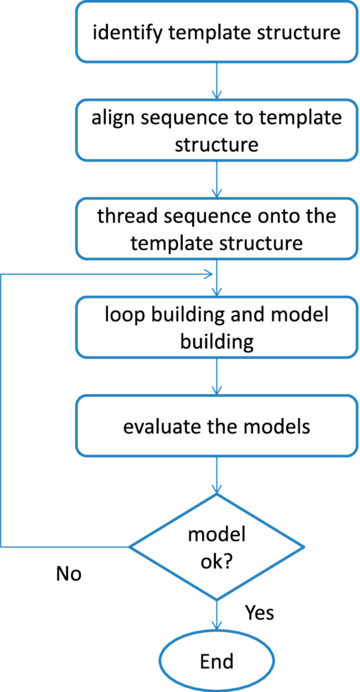
\includegraphics[scale=0.43]{images/homology1.png}
		\caption{Diagramma di flusso della modellazione per omologia. Fonte: \cite{sliwoski2014computational}}
		\label{fig:omologia-flusso}
		\endminipage\hfill
		\minipage{0.48\textwidth}
		\centering
		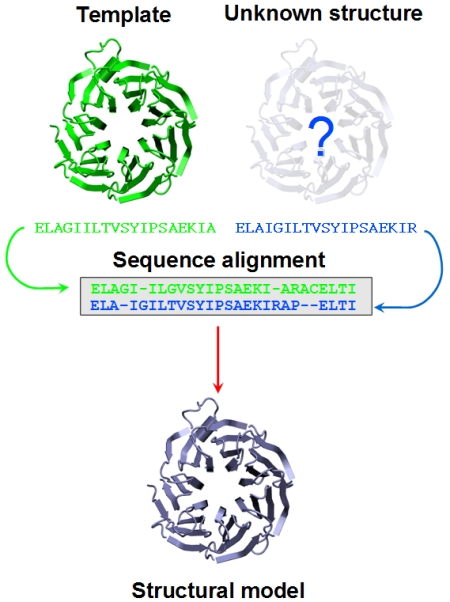
\includegraphics[scale=0.5]{images/homology2.jpg}
		\caption{Schema esemplificativo di una modellazione per omologia. Fonte \cite{UNIL-homology}}
		\label{fig:omologia-esempio}
		\endminipage\hfill
	\end{figure}
	
	Nel 1° step si cerca (almeno) una struttura modello tra le strutture conosciute, avente un'alta somiglianza di sequenza. È più semplice se la struttura di una proteina omologa molto simile è stata già risolta. Ci sono però alcuni gruppi di proteine, come le proteine di membrana, le cui strutture risolte sono scarse. Trovare i giusti template e caratterizzare la loro omologia è ciò che determina in genere il successo dell'intera predizione (una somiglianza minore del 30\% avrà risultati molto scarsi, mentre sopra al 50\% la predizione ha buona probabilità di essere di buon livello). È possibile in ogni caso che vi sia una somiglianza \textit{locale} anche quando la somiglianza globale è scarsa. 
	
	\par Nel 2° step vengono sfruttate informazioni evoluzionistiche per migliorare l'allineamento tra le sequenze dei template e del target. È difficile stabilire allineamenti fra omologhi distanti, come nel caso di target \textit{eucarioti} e template \textit{procarioti}. Altre tecniche usate oltre l'MSA sono: programmazione dinamica, threading, HMM ecc. Possono venire utilizzati più MSA insieme per sopperire a problemi di disallineamento di piccole regioni.
	
	\par Nel 3° step ad ogni segmento della sequenza target viene assegnato un insieme di coordinate spaziali in accordo ai risultati del MSA. Tool noti sono MODELLER (soddisfazione di vincoli spaziali), NEST, COMPOSER e SWISS-Model. La struttura ottenuta potrebbe essere però deformata a causa dell'utilizzo di più template e numerosi inserzioni e cancellazioni. Possono essere presenti lunghezze e angoli dei legami non ottimali e atomi sovrapposti.
	
	\par Per ovviare a tali problemi nello step 4 si applica un processo di raffinamento, specialmente per quanto riguarda i loop (\textit{loop modeling}, vedi sez. \ref{sec: loop-modeling}) e i residui (\textit{side chain modeling}). Vengono applicati algoritmi che confrontano caratteristiche geometriche ed effettuano calcoli energetici che identificano configurazioni atomiche sfavorevoli. 
	
	\par Nel 5° step si valuta l'affidabilità della predizione. Si dice che un modello è affidabile quando è basato su un template corretto e un allineamento approssimativamente corretto. Si può valutare tale affidabilità in vari modi:
	
	\begin{itemize}
		\item alcune qualità della struttura costruita possono essere confrontate con delle tendenze statistiche 
		\item se ci sono vari modelli predetti si calcola l'energia libera e si sceglie la struttura con minor energia libera (ad es. tramite ProSa)
		\item stereochimica (relativa alle proprietà spaziali delle molecole), ad esempio con PROCHECK
		\item la conservazione evoluzionistica a livello amminoacidico può essere correlata con il loro stato "esposto" o "seppellito" (l'idea di partenza è che il nucleo della proteina rimanga inalterato e la superficie sia variabile), ad esempio Profiles3D
		\item se si hanno a disposizione dati sperimentali della struttura nativa della proteina si può validare il modello con la consistenza a essi
	\end{itemize}
	
	\subsubsection{Efficienza e limiti}
	
	Con una somiglianza maggiore del 50\% si registra una RMSD tra 1 e 2 \angstrom, ma è importante notare che non sempre proteine omologhe (vicine sequenzialmente) condividono la stessa funzione e struttura. Un esempio sono le proteine del lievito Gal1 e Gal3: 73\% di identità e 92\% di somiglianza. Queste due proteine hanno però sviluppato differenti funzioni, con Gal1 che è una galattochinasi mentre Gal3 è un induttore trascrizionale\supercite{platt2000insertion}.
	
	\par Non c'è quindi una soglia che assicuri una sicura predizione della struttura: molte proteine con una lontana somiglianza possono svolgere la stessa funzione mentre altre altamente simili possono svolgere funzioni diverse. Una regola empirica è considerare sequenze con più del 30-40\% di somiglianza come sequenze con una struttura o funzione simile.
	
	\begin{figure}[!htb]
		\centering
		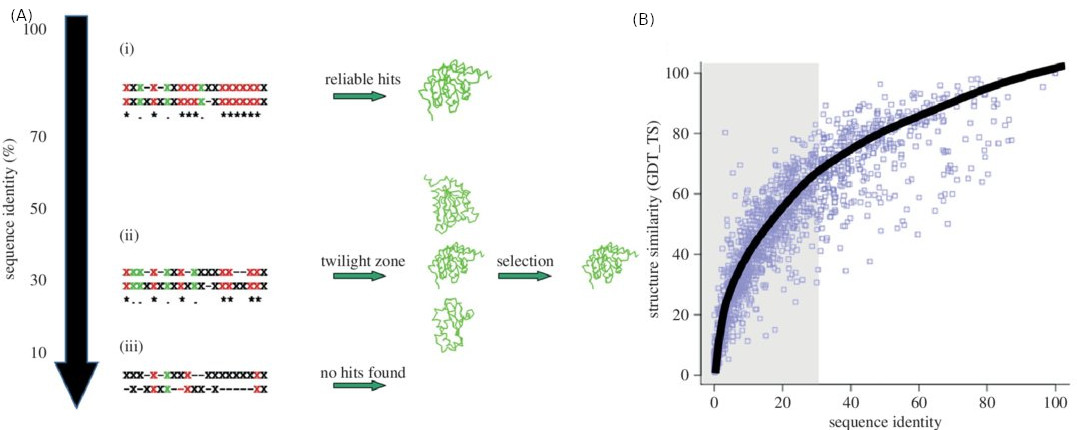
\includegraphics[scale=1.2]{images/homology-grafico.jpg}
		\caption{Risultati dei metodi per omologia alla variazione dell'identità nella sequenza. (A) Dimostrazione schematica dell'uso di metodi di allineamento di sequenze per identificare template. 'X' indica un qualsiasi amminoacido. (i) identità > 70\%: semplici allineamenti di sequenza sono sufficienti per trovare il corretto ripiegamento. (ii) Tra il 20 e il 30\% non sempre è possibile trovare il corretto ripiegamento; è necessario effettuare ulteriori raffinamenti. (iii) a bassi livelli l'utilità di questo metodo è molto bassa. (B) Somiglianza strutturale (in GDT\_TS) al variare dell'identità della sequenza. Anche al 30\% il livello di somiglianza è significativo. Fonte\cite{joseph2014local}}
		\label{fig:omologia-grafico}
	\end{figure}
	
	\par Un'osservazione fondamentale risiede sulle basi in sé del metodo: dato l'affidamento pressoché totale nella modellazione comparativa, la struttura modello è condizionata necessariamente a essere più simile ai template che alla reale struttura nativa della sequenza target, nonostante i vari processi successivi di raffinamento che, data la loro natura approssimativa, non sono perfetti. 
	
	\par I problemi maggiori risultano nelle regioni con bassa somiglianza, come ci si può aspettare. Si sta parlando specialmente dei \textit{loop}, soggetti a mutazioni considerevoli durante l'evoluzione.
	
	\par Si incorrono in problemi con la modellazione per omologia quando si trattano proteine che non hanno omologhe tra le strutture conosciute, come le proteine di membrana, le quali sono difficili da cristallizzare (anche se, come spiegato nella sezione \ref{sec:determinazione-sperimentale}, con la microscopia crioelettronica sta diventando possibile determinare le loro strutture). \\
	
	\par Nonostante tutte le osservazioni fatte, \textit{la modellazione per omologia, quando possibile, è correntemente il miglior metodo computazionale per predire la struttura delle proteine} e la sua applicabilità è destinata a crescere con l'aggiunta di nuove strutture determinate sperimentalmente da poter essere usate come template.
	
	\par Oltre alla PSP i metodi per omologia sono anche usati nel drug design (per studiare le differenze strutturali fra le proteine bersagliate dallo stesso farmaco) e nello studio dei meccanismi catalitici.
	
}

\subsection{\textit{fold recognition}}
{

Come si è già detto la struttura delle proteine è maggiormente conservata rispetto alle sequenze. Questo significa che proteine con differenti sequenze possono ancora formare strutture simili grazie a certe proprietà condivise codificate nelle loro sequenze. Identificando queste proprietà è possibile predire la struttura di una nuova proteina basandosi su un template che condivide le stesse proprietà, anche se loro sequenze sono diverse. Questa è l'idea su cui si basano i metodi di \textit{fold recognition}. Le proprietà di cui si parla sono principalmente le annotazioni già calcolate precedentemente.
In altri termini, in questo approccio si cerca una proteina con struttura conosciuta (nel PDB) che abbia alcune proprietà nella sequenza o tendenze condivise con la proteina target: le due probabilmente hanno un ripiegamento o motivi strutturali simili.

\begin{figure}[!htb]
	\centering
	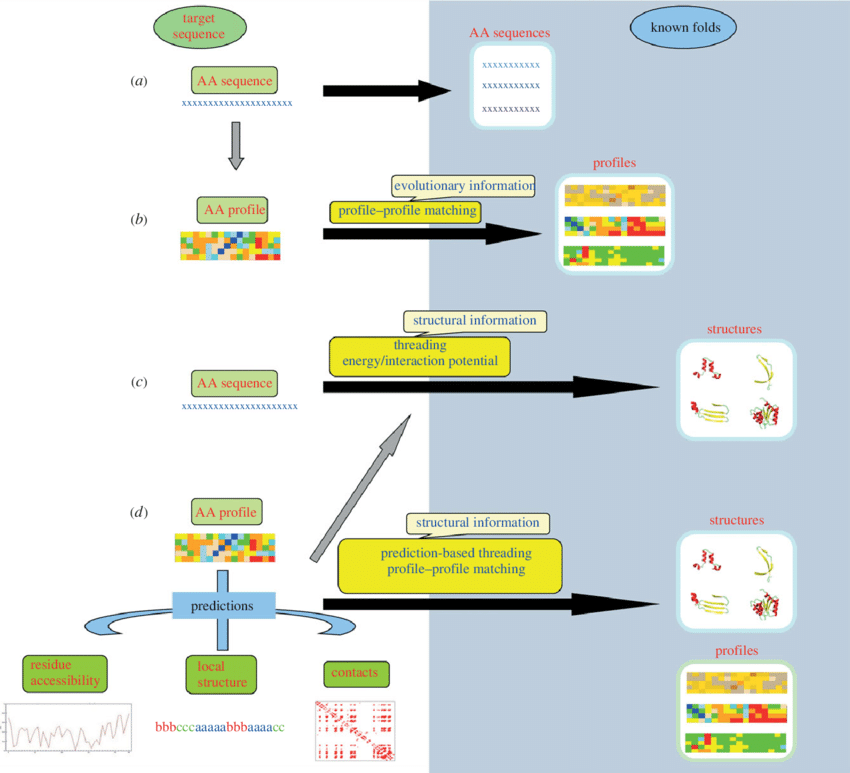
\includegraphics[scale=0.53]{images/threading-mappa.png}
	\caption{Differenti strategie per il fold recognition. A destra, su sfondo blu, c'è l'insieme delle proteine con ripiegamenti conosciuti. La lunghezza delle frecce è correlata alla distanza di relazione fra target e template. Fonte\cite{joseph2014local}}
	\label{fig:fold-recognition}
\end{figure}

È possibile dividere il \textit{fold recognition} in vari livelli a seconda della distanza di omologia che può intercorrere fra la proteina target e il template (come mostrato in fig. \ref{fig:fold-recognition}). Analizzando questa figura si possono descrivere i livelli di ricerca in un tipico algoritmo di \textit{fold recognition}:

\begin{itemize}
	\item (a) \textit{ricerca per sequenza}, ovvero la ricerca iniziale di sequenze omologhe (relazione molto vicina)\footnote{Come accennato nella sezione sulla classificazione dei metodi, il confine tra le varie tecniche è sempre più sfumato. Infatti \textit{homology modeling }e \textit{fold recognition} sono spesso usati insieme come in questo caso, e può essere di aiuto pensare a tale metodo combinato come un \textit{data-based modeling}.}
	\item (b) \textit{profile-profile matching}, vengono aggiunte informazioni evolutive usando il profilo generato nelle annotazioni 1D
	\item (c) \textit{sequence-structure matching}, la sequenza target può essere allineata con strutture di proteine conosciute per valutare la compatibilità (\textit{threading})
	\item (d) \textit{annotation search}, viene effettuata una ricerca confrontando le annotazioni 1D e 2D precedentemente calcolate con le annotazioni di strutture conosciute
\end{itemize}

Nel \textit{profile-profile matching} le proteine i cui profili sono sufficientemente simili alla proteina target possono essere usate come template globali. Un esempio di procedura profile-matching è HHPred, basata su confronti tra coppie di profili HMM target e template, e JACKHMMER. Alcuni studi riportano che i metodi di confronto fra profili basati su HMM siano più efficienti dei profili basati PSSM\supercite{joseph2014local}.

\par Nel \textit{sequence-structure matching} la compatibilità può essere quantificata in base all'interazione globale o al potenziale di energia. È bene notare che la procedura di \textit{threading} può essere difficile e computazionalmente costosa.


\subsection{\textit{ab initio}} \label{sec:ab-initio}
{
Il metodo più lineare e a prima vista ovvio per predire la struttura nativa di proteine è seguire la natura, simulando accuratamente come le forze fisiche guidino la proteina a ripiegarsi e usare questa simulazione per riprodurre il processo di ripiegamento su proteine con strutture sconosciute. \textit{Ab initio}, termine latino, significa infatti "dall'inizio". Questo approccio si basa sul postulato di Anfinsen.

\par Il primo problema che sorge è superare il paradosso di Levinthal. Per farlo si assume un profilo energetico a imbuto del ripiegamento, ovvero la premessa termodinamica che la forma nativa di una proteina sia lo stato in cui risulta avere più bassa energia libera, o più precisamente (richiamando la definizione di struttura nativa data nella sez. \ref{sec:energetica}) quella conformazione avente minore energia libera tale da mantenere il livello di dinamicità richiesto alla proteina per svolgere la sua funzione biologica.

\par Le predizioni nell'approccio \textit{ab initio} sono pertanto \textit{energy-based}, ovvero guidate dall'idea di minimizzare l'energia. Si può vedere il PSP secondo l'approccio \textit{ab initio} come un problema di ottimizzazione dove una funzione di energia gioca il ruolo di \textit{euristica} cercando di raggiungere il minimo globale di energia all'interno dello spazio di ricerca. In quanto \textit{energy-based} usano solo informazioni sul tipo di atomi nel sistema, le loro posizioni relative nello spazio tridimensionale e le loro interazioni con gli altri atomi. Viene poi calcolato l'intero contenuto di energia del sistema e le forze agenti su ogni atomo. 

\par L'energia totale di un sistema (\textit{free energy}) può essere decomposta in varie componenti: cinetica, potenziale, termica ecc. È l'energia libera che determina la stabilità del sistema. Come si vedrà sotto, nell'approccio fisico non viene calcolata tutta l'energia libera ma viene approssimata con una sua parte per motivi di complessità.

\par Sebbene vi siano differenti metodi in questo approccio, tutti condividono due caratteristiche di base:
\begin{itemize}
	\item calcolano il contenuto di energia del sistema in una singola configurazione
	\item campionano numerose configurazioni e ne trovano una con la minor energia libera
\end{itemize}

Per \textit{configurazione} si intende la disposizione complessiva di tutti gli atomi di tutti i componenti del sistema (proteina, solvente, ioni, membrana ecc.) mentre la posizione collettiva dei soli atomi della proteina viene chiamata \textit{conformazione}.

\subsubsection{Molecular mechanics \& dynamics}

\par Per descrivere in maniera affidabile tutte le forze fisiche operanti sul sistema tra i differenti atomi bisognerebbe descriverne la distribuzione di tutti gli elettroni, il che richiede però calcoli di meccanica quantistica (QM). Le forze, in un sistema molecolare, risultano dalla distribuzione spaziale degli elettroni attorno agli atomi. Sfortunatamente questi calcoli sono computazionalmente molto costosi e una rigorosa caratterizzazione di un sistema macromolecolare, con milioni di atomi, è al momento insostenibile. Calcoli di QM su una singola conformazione di una piccola proteina possono richiedere mesi, tempi troppo lunghi se si ha l'obiettivo di provare tante configurazioni per sceglierne una finale. 

\subsubsection{Molecular mechanics}

\par Per le ragioni sopra elencate gli scienziati spesso investigano sistemi macromolecolari usando approssimazioni delle reali forze in essi. Il campo da cui i calcoli per le approssimazioni sono presi è chiamato \textit{molecular mechanics} (MM), poiché approssima sistemi molecolari usando espressioni prese dalla meccanica newtoniana classica:
\begin{itemize}
	\item il contenuto di energia è descritto usando un \textit{campo di forza} nel quale gli atomi e i legami covalenti sono trattati come palline e molle
	\item le descrizioni che richiederebbero calcoli di QM vengono ignorate
	\item le rappresentazioni sono \textit{esplicite}: prendono in considerazione tutti gli atomi (vedi fig. \ref{fig:descrizione-esplicita-mm})
\end{itemize}

Il campo di forza sopra accennato descrive l'energia potenziale del sistema. Da notare che l'energia potenziale (intesa come entalpia) è solo una delle due componenti dell'energia libera, vedi sez. \ref{sec:energetica}).

\par Un campo di forza è un'energia di posizione: l'energia di un oggetto in una specifica posizione all'interno di un campo (gravitazionale, elettrico, magnetico ecc.). Nelle molecole l'energia potenziale è la somma di tutti gli effetti dei campi elettrici atomici\footnote{Gli atomi possiedono, in base alla loro eventuale carica, campi elettrici che influenzano gli altri atomi.} in una determinata posizione. Si può approssimare l'energia potenziale all'energia risultante da tutti i legami covalenti e le interazioni non covalenti, escluse quelle non polari \footnote{Un esempio di interazione non polare è l'effetto idrofobico. Vengono escluse poiché coinvolgono principalmente cambiamenti di entropia nel solvente.}, in una singola configurazione del sistema. In genere i campi di forza non sono una singola funzione ma una somma di più termini, ognuno corrispondente a un differente tipo di legame chimico o interazione, un esempio:

\[ U_{tot}=U_{cov}+U_{elst}+U_{vdw} \]

dove per $U_{tot}$ si intende l'energia potenziale totale, per $U_{cov}$ l'energia potenziale dei legami covalenti, per $U_{elst}$ quella delle interazioni elettrostatiche e per $U_{vdw}$ quella delle interazioni di van der Waals.

\par L'energia potenziale delle interazioni elettrostatiche può essere calcolata con la legge di Coulomb, mentre quella delle interazioni di van der Waals tramite l'equazione di Lennard-Jones. Nelle simulazioni di sistemi biologici vengono usati: CHARMM, AMBER, GROMACS, ecc.

\begin{figure}[!htb]
	\centering
	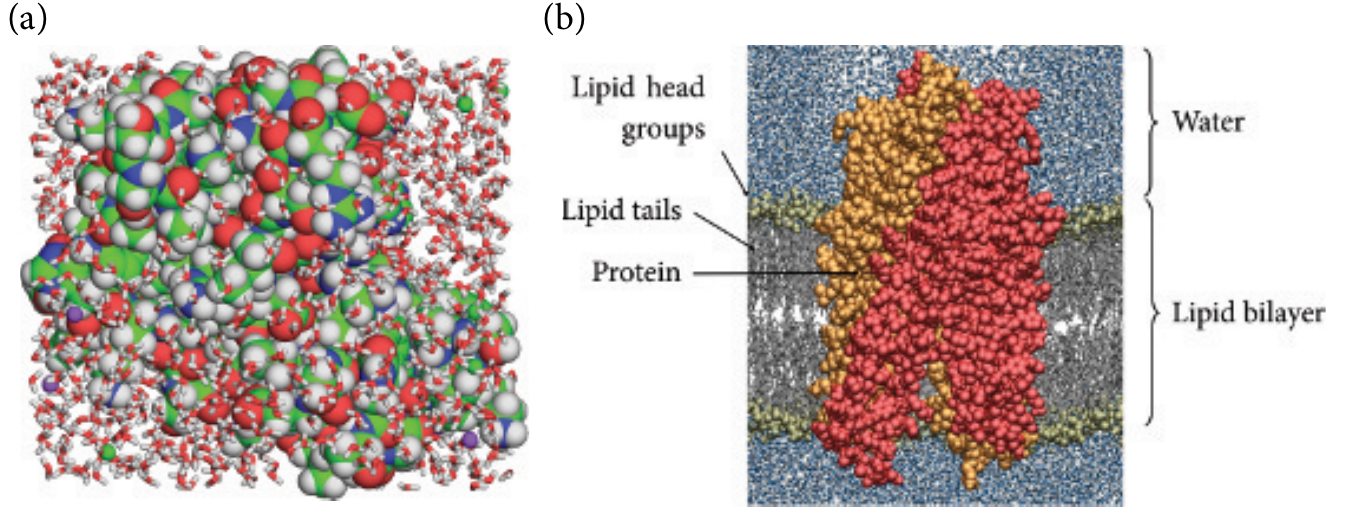
\includegraphics[scale=0.4]{images/esplicita-mm.png}
	\caption{Descrizioni esplicite nei calcoli di MM. (A) una piccola proteina immersa in un solvente composto da molecole d'acqua e ioni (Na$^{+}$, Cl$^{-}$). La proteina è rappresentata come sfere di atomi, l'acqua come bastoncini e gli ioni come piccole sfere magenta e gialle. (B) una proteina trasportatrice in un doppio strato lipidico, circondato da ambiente acquoso. La proteina e le teste dei lipidi sono rappresentate in modo space-fill, mentre l'acqua e le code dei lipidi con rappresentazione wire-frame. Fonte \cite{kessel_ben-tal_2018}}
	\label{fig:descrizione-esplicita-mm}
\end{figure}

\par La descrizione approssimata fornita dal campo di forza permette di calcolare l'energia potenziale di molti sistemi macromolecolari in meno di un secondo. \\

\par Una variante del MM è la \textit{QM/MM} nella quale i calcoli di QM sono indirizzati solamente su una piccola parte della proteina che contiene residui funzionali importanti. Le altre regioni sono soggette invece a MM, con calcoli molto più veloci\footnote{Questo approccio è stato introdotto da Warshel, Levitt e Karplus.}.

\subsubsection{Spazio configurazionale}

\par Assumendo l'accuratezza del campo di forza, il calcolo dell'energia potenziale di un sistema consente di determinare (parte del)la stabilità di una configurazione. L'idea iniziale potrebbe essere quella di considerare tutte le possibili locazioni atomiche del sistema, calcolare l'energia potenziale in ogni caso e scegliere quella con la minor energia. Come si può facilmente intuire ciò risulta essere un procedimento troppo oneroso, in quanto si devono considerare anche gli atomi del solvente (ed eventuali ligandi o cofattori). Anche il solo numero delle possibili configurazioni atomiche è difficile da calcolare.

\par Per superare questo problema vengono usate tecniche per ridurre lo spazio di ricerca nello spazio configurazionale. Ci sono vari metodi di ricerca, ad esempio: \textit{systematic search }(grid search basata su dettagli geometrici), \textit{model-building model }(usa frammenti molecolari), \textit{random approach }(movimenti random sul piano cartesiano da una configurazione iniziale), \textit{distance geometry} (usa una matrice di distanze atomiche), \textit{Monte Carlo method} (modifiche random e accettazione probabilistica di configurazioni a livelli energetici maggiori)\supercite{ROY2015151}.

\par Il metodo più semplice è chiamato \textit{energy minimization}:

\begin{enumerate}
	\item si parte da una configurazione arbitraria
	\item si calcola l'energia potenziale e viene derivato questo valore su differenti posizioni nel sistema in modo da calcolare le forze agenti su ogni atomo dalla rimanente parte del sistema
	\item un piccolo cambiamento è introdotto nella posizione di ogni atomo, in risposta alle forze applicate su ognuno di essi dal resto del sistema (in accordo a quanto calcolato nel precedente step)
	\item se la nuova configurazione ha un'energia minore viene adottata
	\item altrimenti questa viene scartata e viene creata una nuova configurazione
	\item si ritorna allo step 3 finché non si trovano più configurazioni con minor energia
\end{enumerate}

Il metodo passa da una configurazione all'altra scendendo con il gradiente della superficie dell'energia potenziale finché non converge in un \textit{punto di minimo locale}. Tutte le procedure di \textit{energy minimization }tendono spesso a rimanere bloccate in un minimo locale di energia, non riuscendo a raggiungere il minimo globale a causa di \textit{barriere energetiche} da scavalcare per raggiungere una configurazione con energia minore (vedi fig. \ref{fig:energy-minimization} e \ref{fig:imbuto}).

\begin{figure}[!htb]
	\centering
	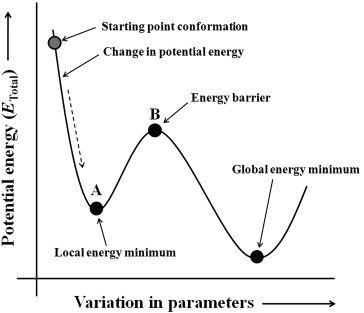
\includegraphics[scale=1]{images/energy-minimzation.jpg}
	\caption{Differenti fasi energetiche di una molecola durante la sua minimizzazione energetica. Fonte\cite{ROY2015151}}
	\label{fig:energy-minimization}
\end{figure}

\subsubsection{Molecular dynamics}

È possibile spingere l'algoritmo di minimizzazione energetica fuori da punti di minimo locale fornendo energia extra, ad esempio innalzando la temperatura del sistema (ovvero aggiungendo calore virtuale). L'energia aggiunta consente agli atomi del sistema di incrementare i loro movimenti e nuove configurazioni fuori dalle barriere energetiche vengono create. Questo metodo è chiamato \textit{Molecular dynamics} (MD) e si focalizza sui movimenti dipendenti dal tempo degli atomi nel sistema. I calcoli sono realizzati in accordo alla meccanica classica. 

\par Agli atomi viene assegnata una velocità iniziale (proporzionale alla temperatura) e continuano a muoversi nello spazio secondo i corrispondenti cambiamenti nell'energia potenziale del sistema. Il movimento di ogni atomo nel sistema è calcolato in base alla sua energia in quel dato momento.

\par Le simulazione di MD sono eseguite in cicli ripetitivi di \textit{riscaldamento} e \textit{raffreddamento} (metodo conosciuto nel mondo informatico come \textit{simulated annealing}, in riferimento al processo di tempra dei metalli). Nella fase di riscaldamento vengono superate le barriere energetiche mentre la fase di raffreddamento (seguita dall'\textit{energy minimization}) consente al sistema di rilassarsi in configurazioni con minor energia.

\par Un metodo comune per rendere la ricerca con MD più efficiente è di spezzarla in due fasi:
\begin{itemize}
	\item ricerca a bassa risoluzione per trovare una collezione di strutture con interazioni non polari (basato sulla nozione che il nucleo delle proteine globulari sia idrofobico)
	\item ricerca ad alta risoluzione fra le strutture selezionate nel primo step
\end{itemize}

\subsubsection{Limiti dell'approccio fisico e parziali soluzioni}
Sebbene simulare il ripiegamento proteico seguendo la meccanica classica possa apparire un approccio attraente, questo è pratico solo per piccole proteine e usando alte risorse computazionali: lo spazio di ricerca è enorme e il problema è computazionalmente intrattabile in modo deterministico (è NP-hard)\supercite{abbass2020enhancing}.

\par I metodi di MM/MD trovano difficilmente impiego in processi biologici rilevanti come il protein folding. Alcuni problemi riguardano l'approssimazione in sé del campo di forza, la sua accuratezza e i possibili doppi conteggi delle forze in gioco (es. interazioni ioniche e legami idrogeno calcolate in due espressioni differenti). 

\par Un altro problema, sempre nell'approssimazione dell'energia libera con campi di forza, è che forniscono sì l'energia potenziale ma non l'entropia. L'unico modo per stimare l'entropia e l'energia libera dai calcoli per l'energia potenziale è eseguire questi calcoli su tutte le possibili configurazioni del sistema e poi integrarli. Il problema risiede quindi nell'impossibilità di compiere la totalità di questi calcoli a causa delle rappresentazioni esplicite usate nelle simulazioni di MD. In particolare è difficile considerare tutte le configurazioni del solvente acquoso. Ciò che si sta calcolando non è l'energia libera ma un \textit{potenziale di forze medie} (PMF). In conclusione le simulazioni di MD non sono consigliate per descrivere gli effetti dei solventi.

\subsubsection{Mean field approach}
Per ovviare parzialmente al problema delle rappresentazioni esplicite è possibile descrivere \textit{implicitamente} parti del sistema che vengono descritte da una proprietà media, per questa ragione tale approccio è chiamato \textit{mean field}. Un esempio è la descrizione del solvente, la parte "meno" interessante in genere, come una massa omogenea descritta dalla sua \textit{dielettricità} \footnote{Proprietà di un mezzo non conduttore di essere sede di un campo elettrostatico.}, conosciuto anche come approccio \textit{continuum-solvent}, vedi fig. \ref{fig:mean-field}.

\begin{figure}[!htb]
	\centering
	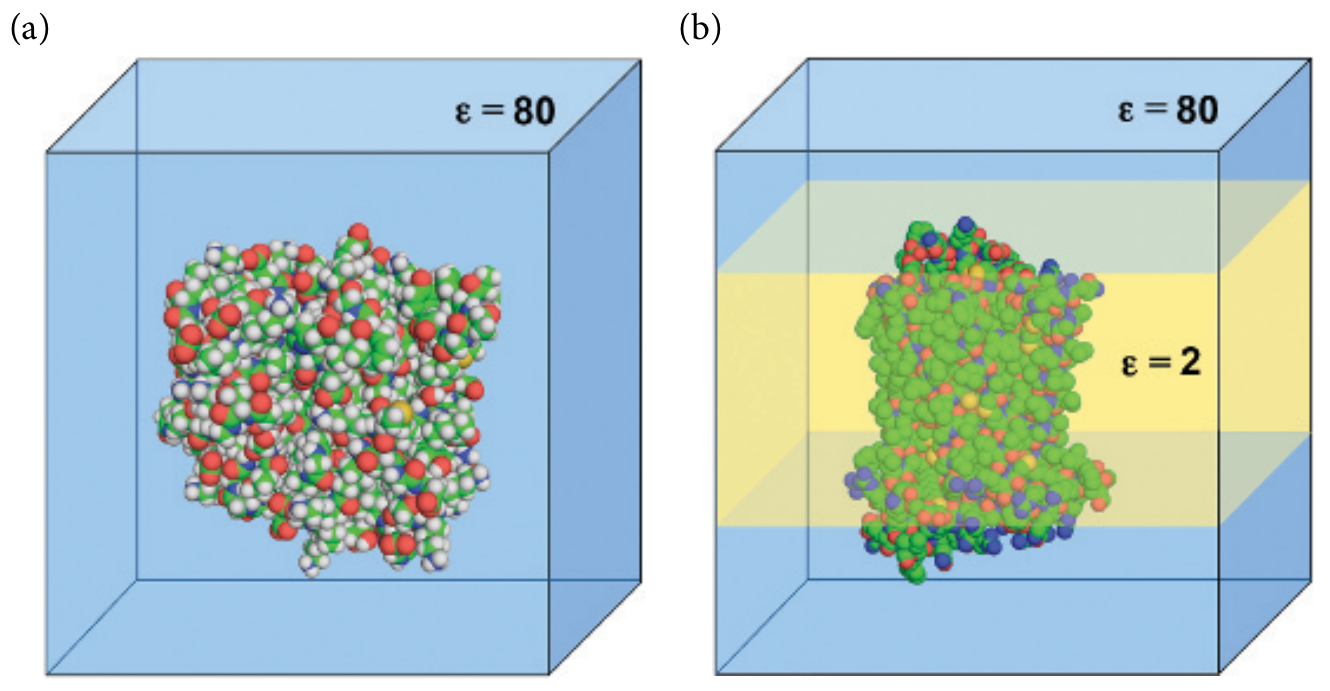
\includegraphics[scale=0.4]{images/mean-field.png}
	\caption{Descrizione con approccio mean-field di un sistema, il solvente è descritto implicitamente mentre la proteina esplicitamente. $\epsilon$ indica la dielettricità. (A) proteina in un solvente acquoso altamente dielettrico. (B) proteina di membrana in un ambiente eterogeneo. Il solvente acquoso è altamente dielettrico mentre la lastra semi-trasparente gialla, che rappresenta la regione biologica di doppio strato lipidico, è poco dielettrica. Fonte\cite{kessel_ben-tal_2018}}
	\label{fig:mean-field}
\end{figure}

Ovviamente, essendo una forte approssimazione, alcuni aspetti del sistema reale sono ignorati, come le interazioni fra gli atomi delle proteine e le molecole d'acqua. Tale problema si esacerba quando il solvente è una membrana. \\

\par Un altro compromesso è l'approccio \textit{mixed force fields} che combina calcoli espliciti sulla proteina e calcoli impliciti sul solvente. Viene usata l'equazione di Poisson-Boltzman (PBE) per calcolare accuratamente l'energia libera elettrostatica, legando così l'effetto polarizzante delle cariche con il loro ambiente. Essendo però un calcolo oneroso viene in genere risolta l'equazione generalizzata di Born (GB). A partire da queste due equazioni, che calcolano la componente elettrostatica dell'energia libera, è possibile calcolare l'intera \textit{free energy}, in modo abbastanza accurato, con calcoli che si rifanno alla surface area (SA, vedi parte finale della sez. \ref{sec:termodinamica-forze-idrofobiche}). 

\par Questi metodi sono chiamati \textit{PBSA} e \textit{GBSA} rispettivamente, e come si è visto permettono un calcolo più preciso dell'energia libera. Questi possono a loro volta essere combinati con la MM per rappresentare anche le interazioni del sistema (\textit{MM-PBSA, MM-GBSA}) e sono oggi largamente utilizzati.

\par Un altro limite computazionale è il lasso temporale che si riesce a coprire. La maggior parte delle proteine si ripiega in microsecondi mentre le simulazioni riescono a coprire tempi che vanno dai pico ai nanosecondi. Grazie ad avanzamenti nelle risorse informatiche sono stati fatti dei passi avanti da questo punto di vista. Un caso interessante è \textit{Anton}, un supercomputer progettato specificatamente per ottimizzare simulazioni di MD capace di coprire 85 $\mu s$ al giorno per un sistema molecolare di 23 000 atomi (180 volte più veloce di qualsiasi computer general-purpose). Altri progressi sono dovuti alla computazione parallela e alla computazione accelerata dalla GPU. Il calcolo distribuito (\textit{grid computing}), ovvero una larga rete di computer personali dedicati volontariamente al completamento di processi, ha permesso alla rete \textit{Folding@Home} (170 000 computer) di simulare l'intero processo di ripiegamento della proteina di legame dell'acetil coenzima A, composta da 86 residui e che richiede 10 $ms$ per ripiegarsi. Un'altra rete distribuita di calcolo è \textit{Rosetta@Home}, con 86 000 nodi e finalizzata al PSP. \\

\subsubsection{Conclusioni sull'approccio \textit{ab initio}}
I metodi \textit{ab initio} non sono attualmente in grado di predire la struttura della maggior parte delle proteine sulla sola base della loro sequenza. Ma sono molto abili nel farlo quando il punto di partenza della predizione è una struttura vicino a quella nativa. Questi metodi sono infatti ampiamente usati per raffinare le strutture grezze ottenute dalle determinazioni sperimentali (vedi sez. \ref{sec:experimentally-guided-prediction}). 

\par Il loro successo dipende ampiamente dall'accuratezza della funzione di energia, dall'efficienza dell'algoritmo di ricerca nello spazio conformazionale e dall'abilità di discernere strutture native da "esche" energeticamente intrappolate.
Nonostante le loro limitazioni i metodi \textit{ab initio} sono di grande interesse perché sono gli unici, in principio, capaci di derivare la vera struttura nativa delle proteine e possono quindi fornire intuizioni importanti per il protein folding problem. Hanno infatti fornito informazioni importanti sulla dinamica delle proteine e sono utilizzati anche nel \textit{protein engineering} e nel \textit{drug discovery}. 

}

\subsubsection{Valutazione \textit{knowledge-based}}
È anche possibile rimpiazzare il campo di forza con una funzione di valutazione \textit{knowledge-based}. Spesso queste funzioni sono composte di espressioni relative alla tendenza statistica di gruppi chimici, amminoacidi o atomi di interagire fra di loro. L'affidabilità della funzione di valutazione dipende dal database su cui si basa. 

\subsection{\textit{fragment-based}}

Laddove non siano disponibili strutture template adatte (\textit{template-free modeling}), l'uso di metodi \textit{fragment-based} diventa l'unica alternativa pratica poiché le tecniche \textit{ab initio} pure richiedono enormi risorse computazionali anche per proteine ​​molto piccole .

\begin{figure}[!htb]
	\centering
	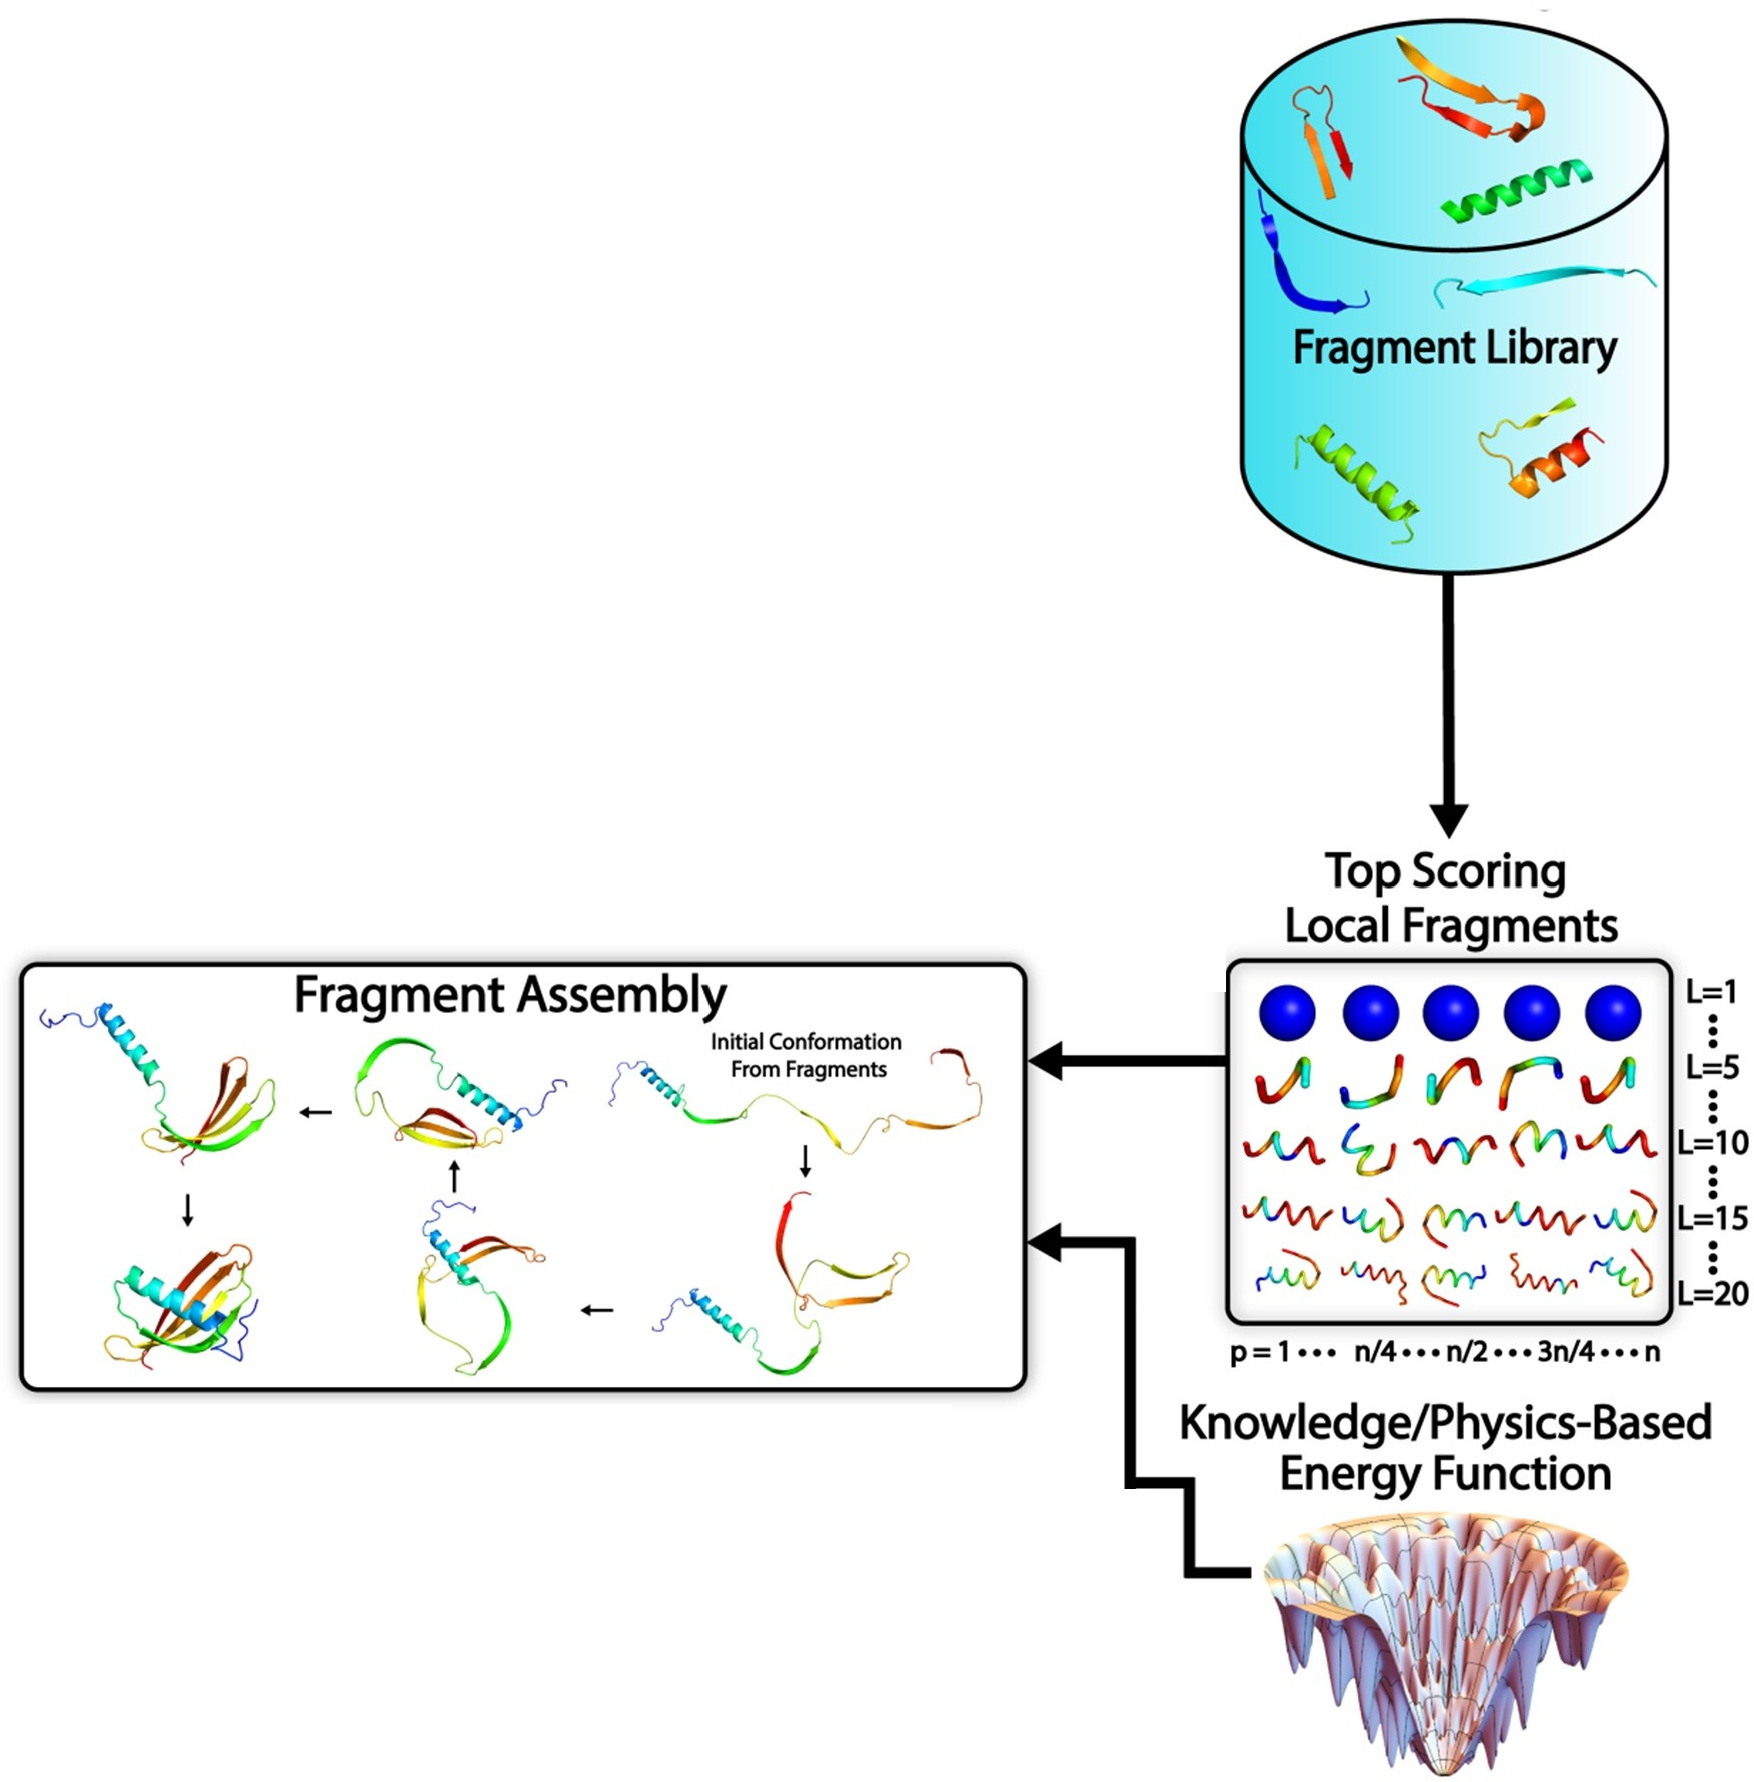
\includegraphics[scale=1]{images/fragment-based.jpg}
	\caption{Step per le tecniche fragment-based nella pipeline generica di un metodo odierno per il PSP. Fonte\cite{pearce2021deep}}
	\label{fig:fragment-based}
\end{figure}

Questi metodi, in primo luogo, ricercano nel PDB frammenti di struttura noti (di pochi residui, ad es. 4-16) che corrispondono a sotto-sequenze della proteina di interesse. Una volta selezionati i frammenti candidati, è possibile formare strutture compatte assemblando frammenti casualmente utilizzando tecniche stocastiche come il \textit{simulated annealing}. Quindi, viene valutata l'idoneità di ciascuna conformazione e vengono ottimizzate quelle più promettenti: mentre i metodi \textit{ab initio} si basano sull'ottimizzazione esplicita dell'energia libera, gli approcci basati sui frammenti svolgono un compito simile utilizzando funzioni di punteggio che sono vagamente correlate alle funzioni energetiche\supercite{abbass2020enhancing}. I metodi fragment-based sono perciò in parte \textit{data-based} e in parte \textit{ab initio}.

\par Inoltre, è stato dimostrato che l'inclusione di una misura di somiglianza tra la struttura secondaria di un frammento candidato e quella prevista nel target migliora le funzioni di punteggio. Per ragioni di ottimizzazione, anche in questi metodi vengono usate le annotazioni 1D e 2D calcolate precedentemente.

\par In questo approccio l'assemblaggio della proteina è quindi realizzato usando piccoli frammenti di proteine conosciute che verranno poi integrati. Un metodo più efficiente rispetto a cercare frammenti nel PDB risulta essere usare librerie di frammenti. Una recente libreria basata sul DL è DeepFragLib. Un principio chiave alla base del PSP \textit{fragment-based} è che qualsiasi struttura può essere costruita dalla concatenazione di frammenti ottenuti da strutture proteiche disponibili nel PDB, per tale ragione una libreria di frammenti ideale dovrebbe essere in grado di costruire qualsiasi proteina. \\


\par Gli approcci basati sui frammenti sono molto meno dispendiosi dal punto di vista computazionale di quelli "classici" ab initio per tre ragioni principali\supercite{abbass2020enhancing}: 
\begin{itemize}
	\item sono \textit{coarse grained} (a grana grossa), l'unità di calcolo è un insieme di amminoacidi anziché uno singolo e ciò diminuisce drasticamente lo spazio di ricerca conformazionale
	\item si utilizzano simulazioni Monte Carlo (MC) al posto della MD
	\item poiché i frammenti utilizzati sono già a bassa energia, non è necessario calcolare le interazioni locali all'interno del frammenti che vengono introdotti nella struttura
\end{itemize}

Per far fronte all'ampio spazio di ricerca, la maggior parte dei metodi \textit{fragment-based} si basano sulla generazione di migliaia di strutture candidate, note come \textit{esche}. Ciascuna di esse rappresenta, in linea di principio, una diversa traiettoria di ricerca. Tipicamente, le esche con il punteggio di energia più basso sono considerate come le migliori previsioni. 

\par Il successo di metodi \textit{fragment-based} per il PSP si basa su tre fondamenti: 
\begin{itemize}
	\item accuratezza della funzione energetica
	\item efficienza del metodo di ricerca 
	\item qualità della libreria di frammenti
\end{itemize}

Esempi di metodi moderni \textit{fragment-based} sono FRAGFOLD, I-TASSER, QUARK e Rosetta.


\subsection{\textit{loop modeling}} \label{sec: loop-modeling}
{
I loop sono regioni della struttura proteica con ruoli spesso cruciali (interazioni con altre proteine, siti di legame con molecole ecc.). Allo stesso tempo sono molto variabili nella loro sequenza e struttura rispetto alle altre regioni. Si trovano generalmente sulla superficie delle proteine e le loro strutture sono note per essere difficili da predire.

\begin{figure}[!htb]
	\minipage{0.48\textwidth}
	\centering
	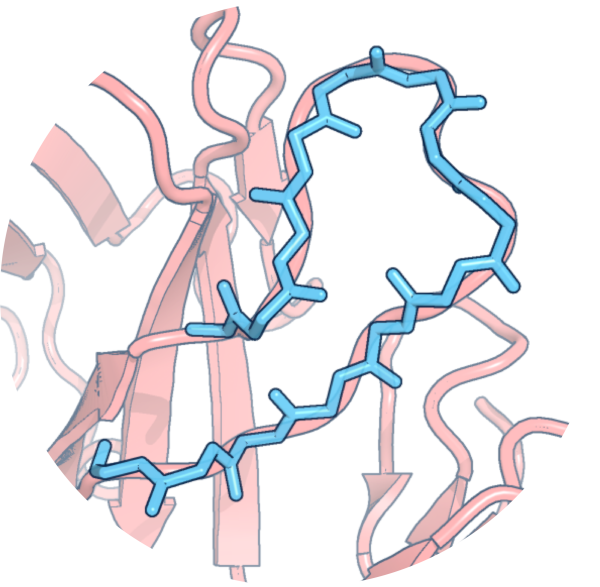
\includegraphics[scale= 1]{images/fread.png}
	\caption{Disegno di un loop in celeste. Fonte \cite{FREAD}}
	\label{fig:loop-example}
	\endminipage\hfill
	\minipage{0.5\textwidth}
	\centering
	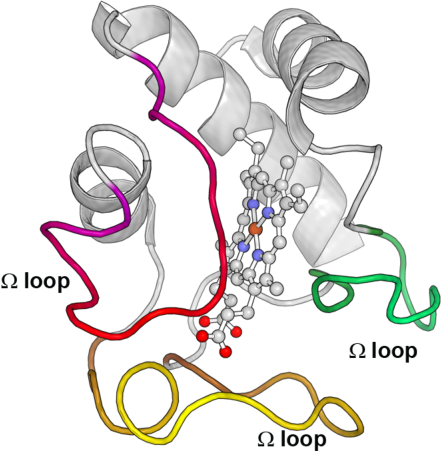
\includegraphics[scale=0.3]{images/loops.png}
	\caption{Omega loop. Sono spesso coinvolti nel riconoscimento molecolare e in funzioni regolatrici. Fonte: \cite{Papaleo2016TheRO}}
	\label{fig:omega-loops}
	\endminipage\hfill
\end{figure}

Il loop modeling non si applica solamente alla fase di raffinamento della modellazione per omologia della predizione di strutture proteiche. È importante anche nella predizione di frammenti mancanti nelle strutture determinate sperimentalmente. È stato stimato che in più della metà delle struttura depositate nel PDB ci siano segmenti mancanti, spesso loop\supercite{karami2018dareus}.

\par Problemi comuni nel loop modeling sono: decidere quale regione del modello sarà un loop; trovare il corretto allineamento di regioni di ancoraggio; la modellazione in sé del loop; le conformazioni di loop multipli, ecc.

\par Nella modellazione per omologia (nel PSP) si registrano spesso grandi deviazioni dai template omologhi: la modellazione dei loop rimane un problema aperto nella modellazione per omologia della struttura delle proteine\supercite{karamiLoop}. Le principali strategie per il loop modeling sono le stesse di quelle per la predizione dell'intera struttura:
\begin{itemize}
	\item \textit{data-based} (o knowledge-based), basati sull'assunzione di similarità sequenza-struttura, ovvero che loop con sequenze simili hanno anche conformazioni simili
	\item \textit{ab initio}, in cui viene esplorato lo spazio conformazionale
	\item approccio ibrido
\end{itemize}

\par Un protocollo comune per la modellazione, partendo da un modello della proteina senza loop e la sequenza del loop, è quello mostrato in figura \ref{fig:loop-modeling-approaches}, con i seguenti step:
\begin{itemize}
	\item generazione di tutti i possibili stati del loop (ab initio, data-based o ibrido)
	\item valutazione e raggruppamento
	\item raffinamento
\end{itemize}

\begin{figure}[!htb]
	\centering
	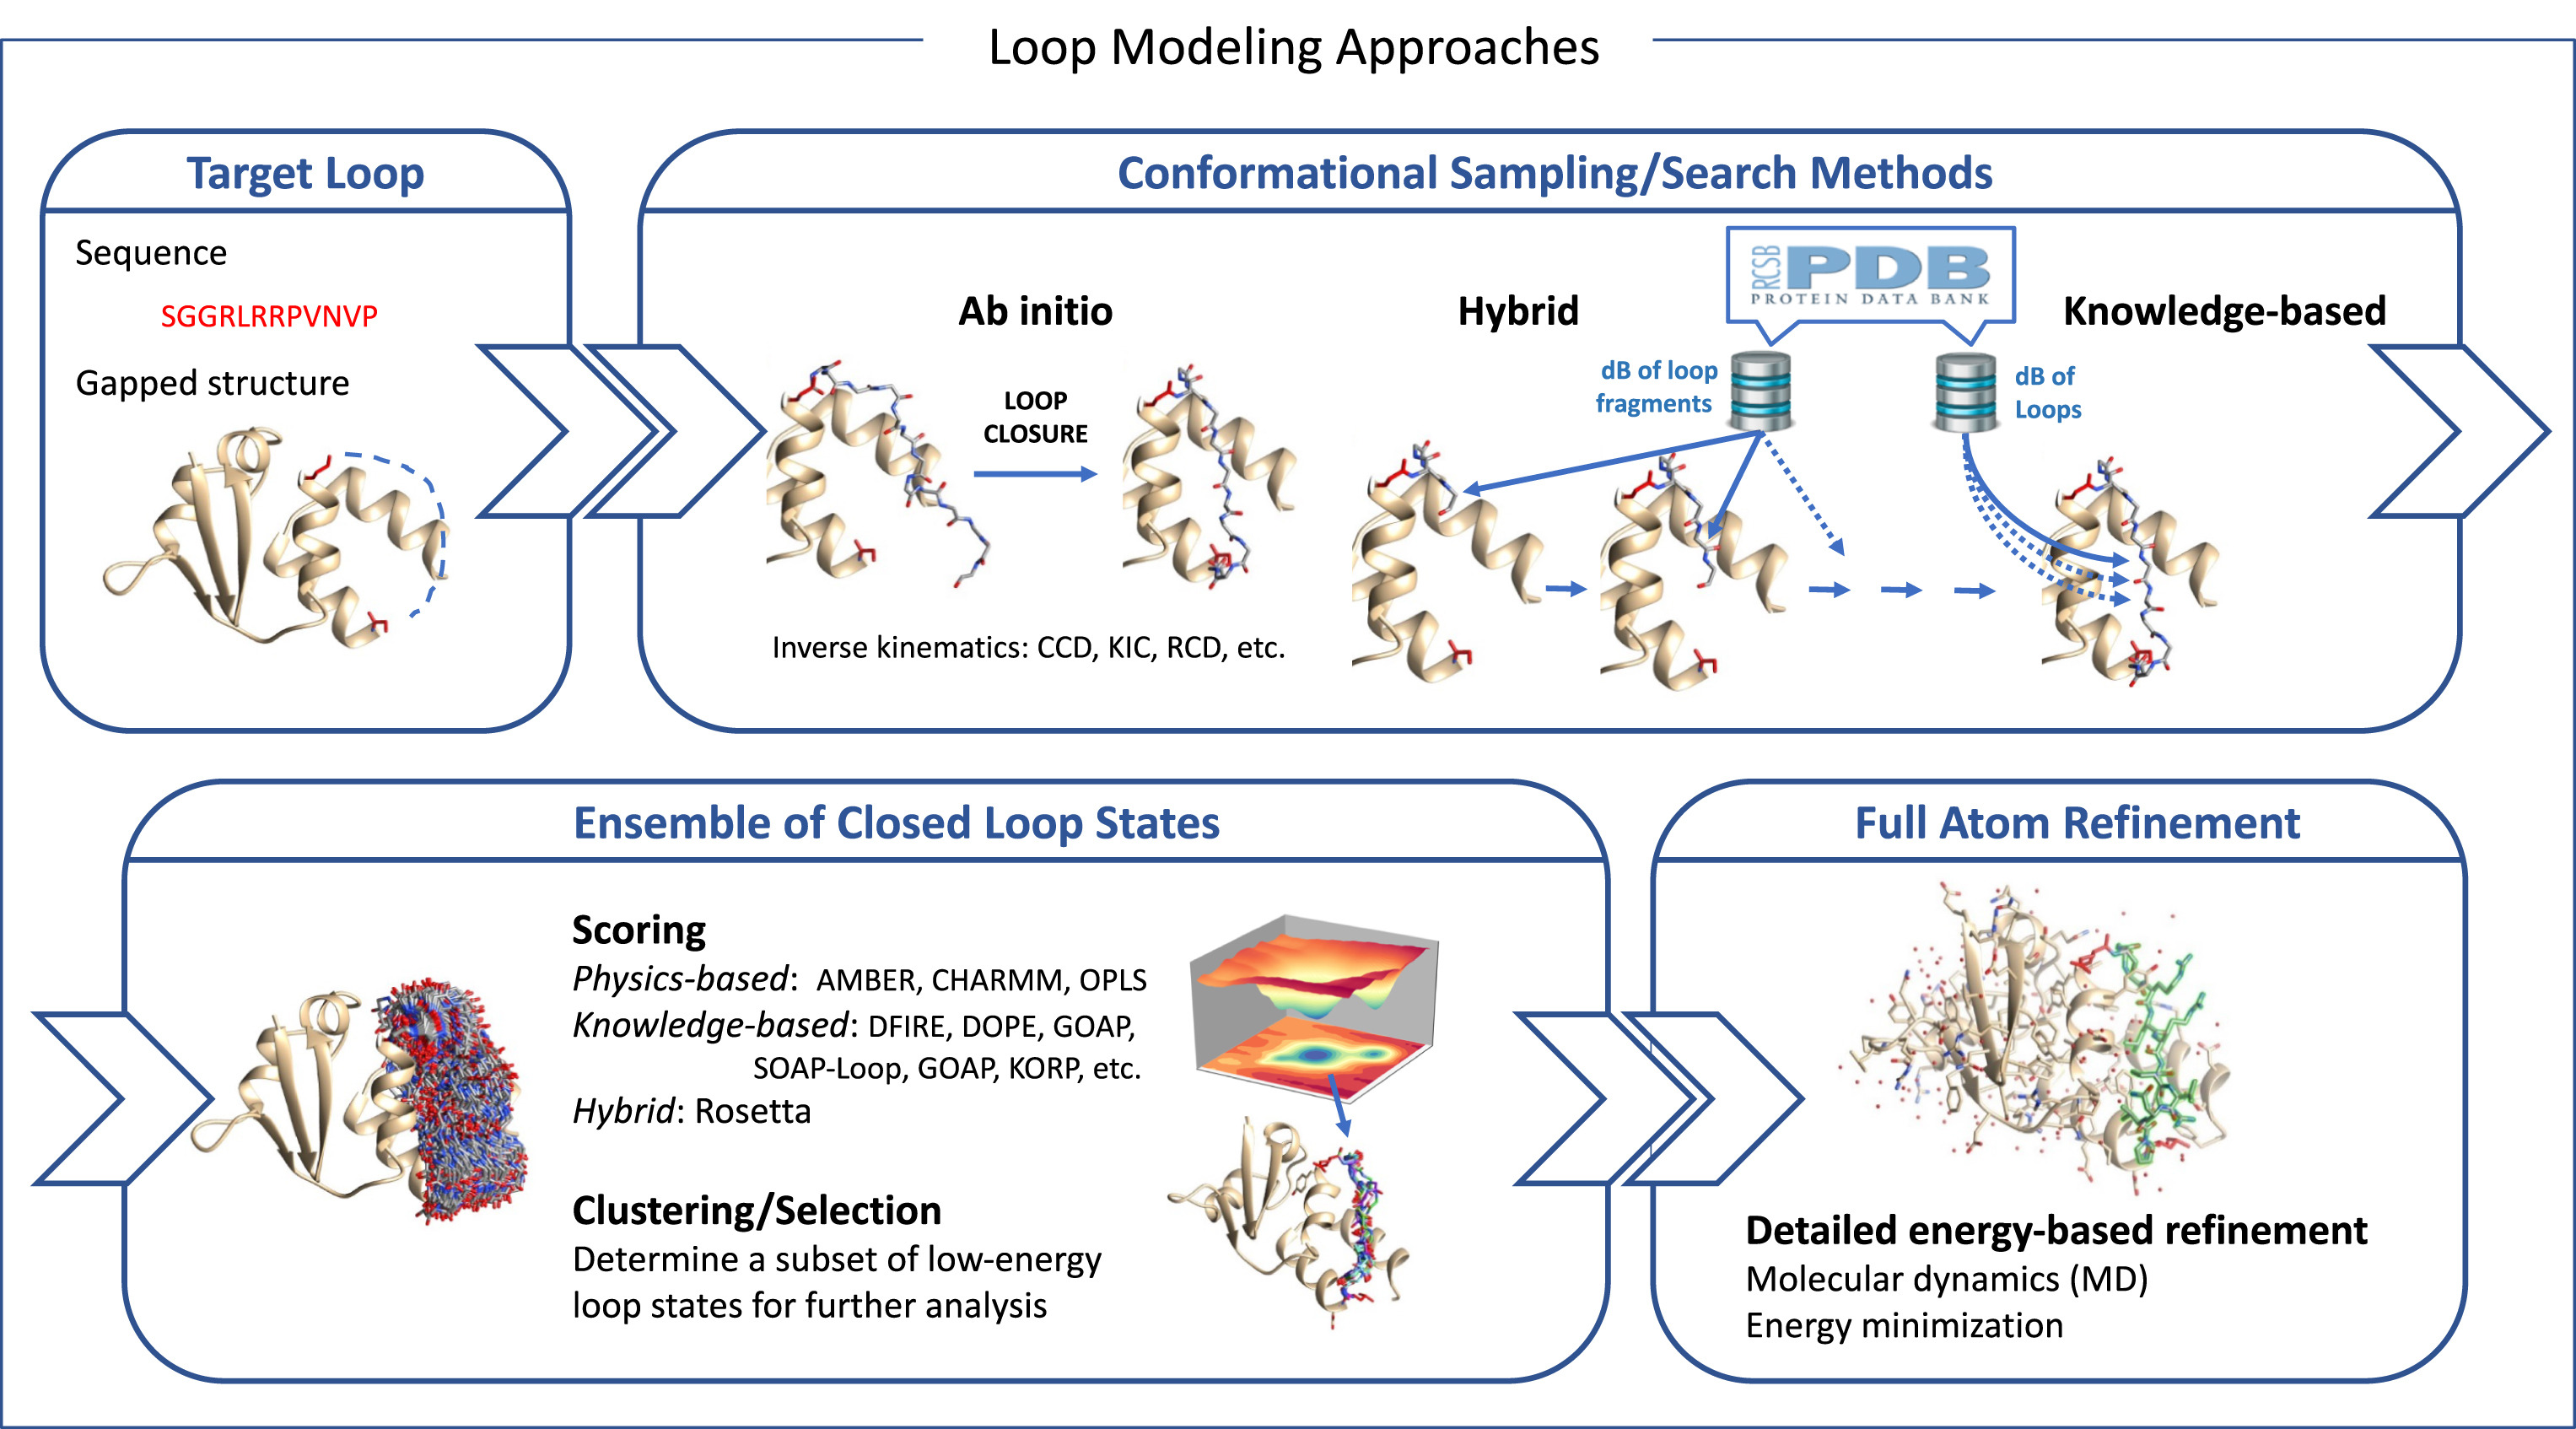
\includegraphics[scale=1]{images/loop-modeling-approaches.jpg}
	\caption{Approcci al loop modeling. Workflow schematico di un protocollo prototipo per la modellazione dei loop. Fonte\cite{barozet2021current}}
	\label{fig:loop-modeling-approaches}
\end{figure}

La ricerca su database è efficiente per famiglie specifiche ma i loop più lunghi di 4 residui devono essere comunque ottimizzati. I residui ai fianchi della regione del loop sono chiamati residui di \textit{ancoraggio} e sono utilizzati per effettuare la ricerca nei database. ArchPRED ad esempio considera le strutture secondarie ai fianchi del loop mancante, il loro orientamento relativo e il numero di residui mancanti per identificare conformazioni del loop candidate. È possibile usare una funzione di valutazione basata sull'energia per valutare la modellazione dei loop, ad esempio basata sulla stereochimica (come in CHARMM). 

\par Molti dei metodi raggiungono ottimi risultati per la predizione dei loop su strutture sperimentali in ambienti esatti (ovvero strutture cristallizzate a cui mancano le regioni dei loop). Ma nei modelli per omologia non si è ancora riusciti a raggiungere buoni risultati\supercite{karami2018dareus}. Metodi allo stato dell'arte sono in grado di predire conformazioni stabili di loop relativamente corti (fino a 12 residui)\supercite{barozet2021current}.
Pur con le loro limitazioni, gli approcci correnti sono pronti per essere usati in problemi impegnativi come il loop design in enzimi e anticorpi.

\par I metodi \textit{ab initio} sono dipendenti dalle tecniche di ottimizzazione dell'energia e per questa ragione risultano essere lenti. Metodi \textit{ab initio} per il completamento della struttura cristallizzata allo stato dell'arte sono Rosetta-NGK e GalaxyLoop-PS2. CODA è un esempio di metodo ibrido che combina i due approcci nel loop modeling, così come Sphinx il quale prima esegue una ricerca data-based per trovare frammenti più corti del loop di interesse in modo da ottenere informazioni strutturali, successivamente applica metodi \textit{ab initio} per generare frammenti della corretta lunghezza. \\

\par Pochi metodi sono disponibili come web servers e quindi utilizzabili anche dai non esperti: GalaxyLoopPS2, LoopIng, Sphnix e DaReUS-Loop. Metodi locali sono invece MODELLER, Loopy, OSCAR-loop, Rosetta-NGK, LEAP e M-DISGro. Sono disponibili anche dei tool per la modellazione di loop specifici per gli anticorpi, come quelli offerti da SAbPred\footnote{Collezione di tool sviluppati da Oxford Protein Informatics Group (OPIG).}: Sphinx e FREAD (knowledge-based) che effettua una ricerca su database tenendo in considerazione i vincoli spaziali dei residui di ancoraggio.

\par Possono essere utilizzati anche simulazioni Monte Carlo e MD per investigare proprietà termodinamiche e cinetiche dei loop. Per quanto riguarda l'utilizzo di Deep Learning o Machine Learning per la modellazione dei loop, resta da dimostrare la capacità dei metodi ML/DL di generare modelli significativi di loop flessibili, nonostante in altre aree della bioinformatica strutturale si sia rivelato uno scenario con grande potenziale\supercite{barozet2021current}.

\par Uno dei metodi più recenti e con migliori risultati è DaReUS-Loop, un approccio  \textit{data-based} che identifica loop candidati estraendoli dal completo insieme delle strutture conosciute del PDB. 

\begin{figure}[!htb]
	\centering
	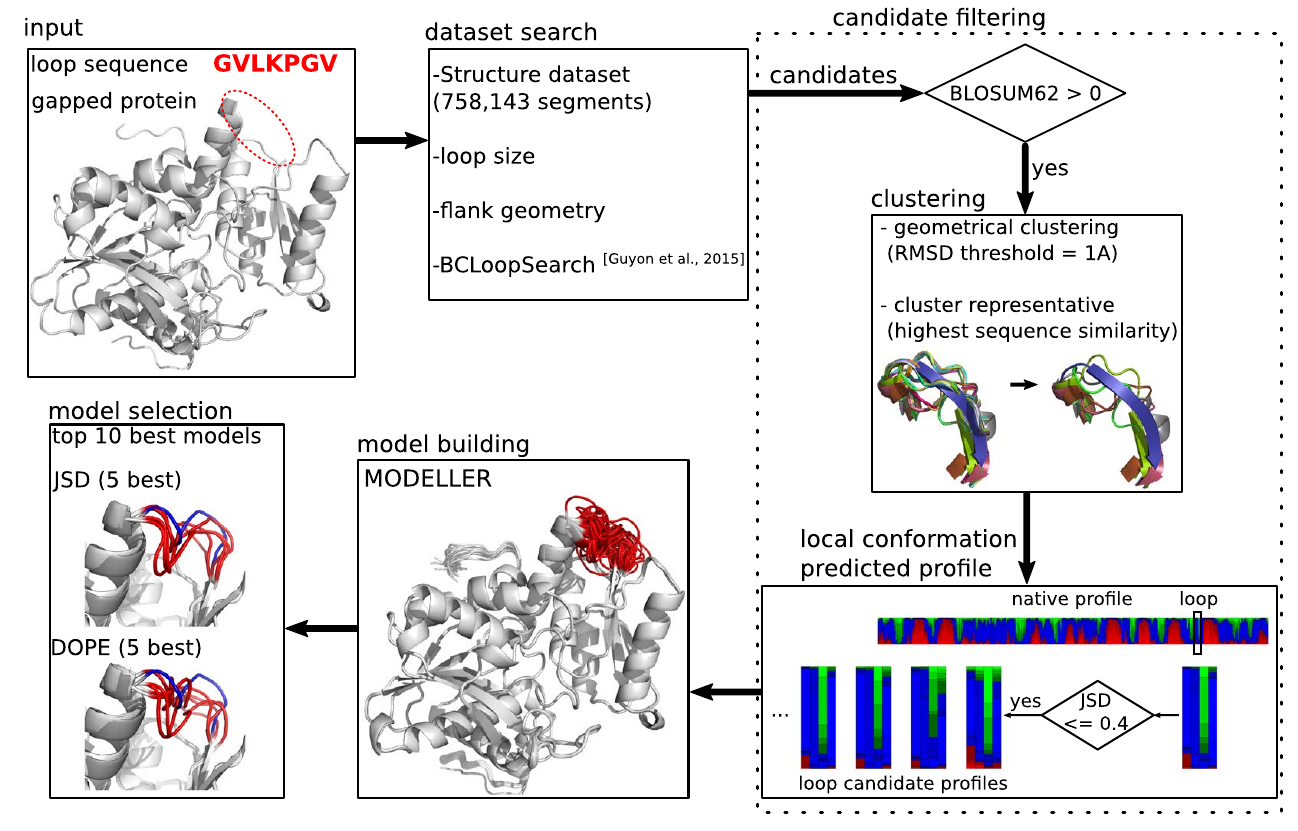
\includegraphics[scale=0.45]{images/dareus.png}
	\caption{DaReUS-Loop workflow. Da notare che dal 2019\supercite{karamiLoop} nel processo di costruzione del modello non è più usato MODELLER (non free) ma GROMACS. Fonte\cite{karami2018dareus}}
	\label{fig:dareus-workflow}
\end{figure}

Il filtraggio dei candidati si basa su confronti di conformazioni locali profilo-profilo insieme a una valutazione fisico-chimica. Applicato ai dataset del CASP11 e CASP12 mostra significativi progressi nell'accuratezza della predizione dei loop e propone una misura di confidenza che correla bene con l'accuratezza effettiva dei loop. I loro autori mostrano anche che oltre il 50\% dei modelli ben riusciti sono derivati da proteine non correlate: ciò suggerisce che frammenti di proteine, sotto simili vincoli, tendono ad adottare simili strutture (oltre la mera omologia)\supercite{karami2018dareus}. 

\begin{figure}[!htb]
	\centering
	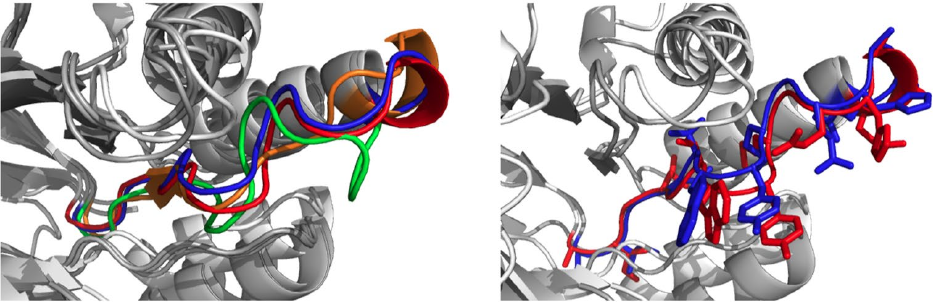
\includegraphics[scale=0.63]{images/dareus-confronto.png}
	\caption{Esempi di predizione di un loop lungo (15 residui) della proteina target T0807 del CASP11 a confronto. Blu=DaReUS-Loop, verde=Rosetta NGK, arancione=GalaxyLoop-PS2, rosso=struttura cristallizzata. La RMSD di ogni loop predetto rispetto al loop nativo è riportata di seguito. DaReUS-Loop: 1.3 \angstrom, NGK: 3 \angstrom, PS2: 2.9 \angstrom. Nella colonna a destra sono riportate le catene laterali della struttura nativa e di quella predetta da DaReUS-Loop. Fonte\cite{karami2018dareus}}
	\label{fig:loop-prediction-lungo}
\end{figure}

I principali step del metodo sono mostrati in figura \ref{fig:dareus-workflow} e sono:
\begin{itemize}
	\item ricerca dei candidati del loop
	\item filtraggio dei candidati
	\item costruzione del modello
	\item model selection
\end{itemize}

Nell'ultimo step sono utilizzate 2 misure per valutare i modelli e vengono ritornati in output come predizioni finali i 5 migliori modelli per ogni metrica.



}

\subsection{Case Study: \textit{TASSER}}

Un metodo che combina differenti approcci (\textit{threading}, \textit{fragment-based} e \textit{ab initio}) è TASSER (Threading/ASSEmbly/Refinement) sviluppato dal gruppo Zhang nel 2004 (negli anni ha subito vari miglioramenti). Il metodo TBM di maggior successo nel CASP è stato probabilmente I-TASSER, l'estensione iterativa di TASSER. Si è infatti costantemente classificato come il miglior metodo automatizzato nel CASP\supercite{pearce2021deep} considerando tutti i target, e anche nel CASP13 e 14, pur non competendo con AlphaFold, ha ottenuto ottimi risultati. È applicabile sia a situazioni TBM che FM in quanto non impone limiti alla lunghezza dei frammenti utilizzati (>5 residui).

\par I-TASSER genera inizialmente conformazioni a bassa risoluzione che sono poi rifinite; la sua pipeline di può essere riassunta nei seguenti 3 step\supercite{abbass2020enhancing}:

\begin{itemize}
	\item \textit{threading}
	\begin{itemize}
		\item vengono identificati i modelli di ripiegamento per la proteina target nella libreria di file utilizzando LOMETS
		\item il threading utilizza un profilo di sequenza e assegnazioni di struttura secondaria, entrambi calcolati dalla sequenza della proteina target
		\item ogni modello è classificato in base a una varietà di punteggi basati sulla sequenza e sulla struttura e i template con punteggi migliori vengono selezionati per il prossimo step
	\end{itemize}
	
	\item \textit{assemblaggio strutturale}
	
	\begin{itemize}
		\item viene assemblata la struttura a grana grossa (senza gruppi laterali)
		\item vengono asportati frammenti dalle regioni maggiormente allineate dei template selezionati
		\item le regioni non allineate (principalmente loop) sono costruite \textit{ab initio}
		\item gli assemblaggi sono eseguiti attraverso simulazioni replica-exchange Monte Carlo (REMC) e vincolati da un campo di forza combinato \textit{energy-based} e \textit{knowledge-based} che include vincoli derivati dal PDB e dal threading 
		\item le conformazioni sono strutturalmente raggruppate per produrre un insieme di rappresentanti: i \textit{cluster centroids}
	\end{itemize}
	
	\item \textit{model selection e raffinamento}, quelle strutture sono raffinate durante un'altra fase di simulazione per produrre tutti gli atomi del modello
	
\end{itemize}

\begin{figure}[!htb]
	\centering
	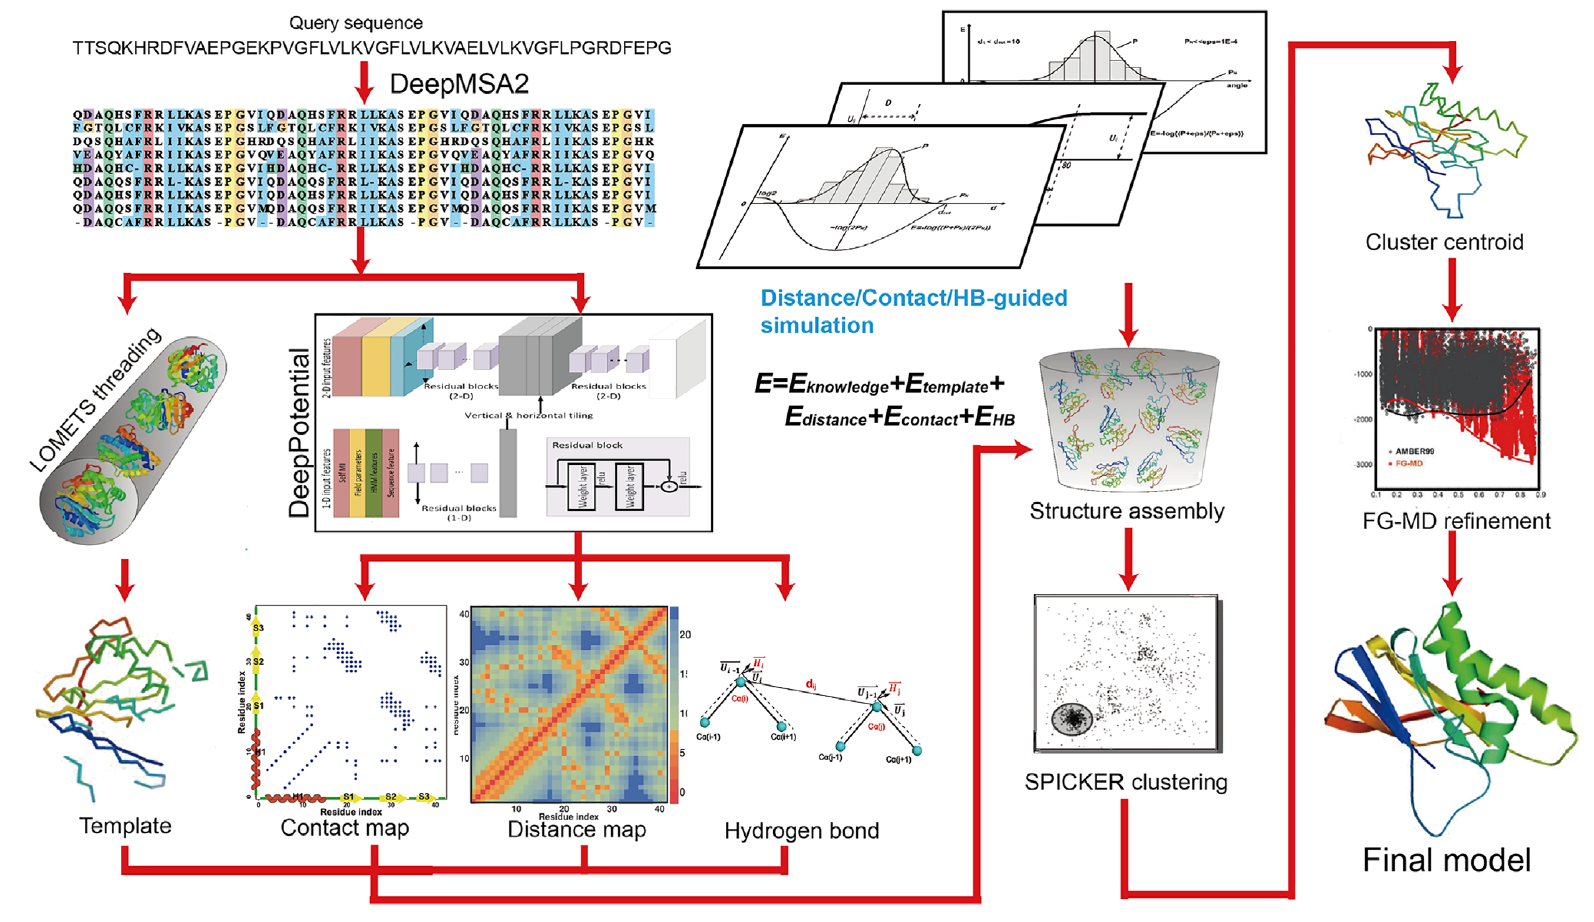
\includegraphics[scale=0.38]{images/DITasser.png}
	\caption{D-I-TASSER pipeline. Fonte\cite{zheng2021protein}}
	\label{fig:DITasser}
\end{figure}

\par Una delle ragioni principali del successo di I-TASSER, in particolare sul perfezionamento dei modelli, è la sua combinazione efficace di più modelli di \textit{threading }(spesso più di 20–50) sotto la guida di un campo di forza combinato \textit{energy-based} e \textit{knowledge-based} ottimale i cui parametri sono stati ampiamente ottimizzati utilizzando richiami strutturali su larga scala. \\

\par Recentemente lo stesso gruppo di ricerca ha sviluppato C-I-TASSER (Contact-Iterative-TASSER), che aggiunge la predizione dei contatti tramite DL, e D-I-TASSER (la cui struttura è riportata in figura \ref{fig:DITasser}), il quale integra la predizione di distanze e legami idrogeno basata su metodi di DL con simulazioni iterative di assemblaggio di frammenti.

Lo stesso gruppo Zhang, nel 2012, ha sviluppato un altro metodo dedicato alla modellazione \textit{ab initio}: QUARK. Questo metodo sfrutta i punti di forza di I-TASSER e Rosetta: oltre al profilo di sequenza e alla struttura secondaria, QUARK utilizza anche l'accessibilità ai solventi e gli angoli di torsione per selezionare piccoli frammenti di dimensioni fino a 20 residui (come Rosetta ma a differenza di I-TASSER), utilizzando un metodo di threading per ciascun frammento di sequenza.

\clearpage